%%%%%%%%%%%%%%%%%%%%%%%%%%%%%%%%%%%%%%%%%%%%%%%%%%%%%%%%%%%%
%% $Id: book.tex,v 1.7 2010/01/11 03:36:49 apollo Exp apollo $
%% $Ver: $
%%%%%%%%%%%%%%%%%%%%%%%%%%%%%%%%%%%%%%%%%%%%%%%%%%%%%%%%%%%%
%\documentclass[10pt]{book}
\documentclass[10pt,dvipdfmx,letterpaper]{report}
%\documentclass[10pt]{report}
\usepackage[dvipdfm,left=1in,right=0.75in,top=1in,bottom=1in]{geometry}
\usepackage{amsmath}
\usepackage{makeidx}
%%%%% For the skak/etc. packages, need ps-tricks, dvi2ps->ps2pdf etc.
% need 'lambda' package - not working on miktex at the moment...
%%\usepackage{skak}
%\usepackage{xskak}
%%%%%
%\usepackage{chessboard}
%%%%%
%\usepackage{diagram}
%%%%%
\usepackage{epic}
%\usepackage[all]{xy}

\usepackage{tikz}
%% for hex grid pattern version 3
%\usetikzlibrary{shapes}
%% for hex grid pattern version 2
%\usetikzlibrary{patterns}
%\def\hexagonsize{0.5cm}
%\pgfdeclarepatternformonly
%  {hexagons}% name
%  {\pgfpointorigin}% lower left
%  {\pgfpoint{3*\hexagonsize}{0.866025*2*\hexagonsize}}%  upper right
%  {\pgfpoint{3*\hexagonsize}{0.866025*2*\hexagonsize}}%  tile size
%  {% shape description
%   \pgfsetlinewidth{0.4pt}
%   \pgftransformshift{\pgfpoint{0mm}{0.866025*\hexagonsize}}
%   \pgfpathmoveto{\pgfpoint{0mm}{0mm}}
%   \pgfpathlineto{\pgfpoint{0.5*\hexagonsize}{0mm}}
%   \pgfpathlineto{\pgfpoint{\hexagonsize}{-0.866025*\hexagonsize}}
%   \pgfpathlineto{\pgfpoint{2*\hexagonsize}{-0.866025*\hexagonsize}}
%   \pgfpathlineto{\pgfpoint{2.5*\hexagonsize}{0mm}}
%   \pgfpathlineto{\pgfpoint{3*\hexagonsize+0.2mm}{0mm}}
%   \pgfpathmoveto{\pgfpoint{0.5*\hexagonsize}{0mm}}
%   \pgfpathlineto{\pgfpoint{\hexagonsize}{0.866025*\hexagonsize}}
%   \pgfpathlineto{\pgfpoint{2*\hexagonsize}{0.866025*\hexagonsize}}
%   \pgfpathlineto{\pgfpoint{2.5*\hexagonsize}{0mm}}
%   \pgfusepath{stroke}
%  }


\usepackage{xcolor}
\definecolor{darkgray}{rgb}{0.25,0.25,0.25}
\definecolor{gray}{rgb}{0.5,0.5,0.5}
\definecolor{lightgray}{rgb}{0.75,0.75,0.75}

\makeindex

\newcommand{\ab}{{$\alpha\beta$}}
\newcommand{\g}[1]{{\sc{#1}}\index{{\sc{#1}}}}
\let\x=\times

%%%%%%%%%%%%%%%%%%%%%%%%%%%%%%%%%%%%%%%%%%%%%%%%%%%%%%%%%%%%
\begin{document}
%%%%%%%%%%%%%%%%%%%%%%%%%%%%%%%%%%%%%%%%%%%%%%%%%%%%%%%%%%%%

\tableofcontents

%%%%%%%%%%%%%%%%%%%%%%%%%%%%%%%%%%%%%%%%
%%%%%%%%%%%%%%%%%%%%%%%%%%%%%%%%%%%%%%%%
%%%%%%%%%%%%%%%%%%%%%%%%%%%%%%%%%%%%%%%%
%%%%%%%%%%%%%%%%%%%%%%%%%%%%%%%%%%%%%%%%
\part{Foundations}

%{
%%%%xskak:
%\newchessgame
%\mainline{1. e4 e5  2. Nf3 Nc6  3. Bb5 a6  4. Ba4 Nf6}
%xskakset{moveid=2w}%
%\chessboard[setfen=\xskakget{nextfen}]\\[1ex]
%Position after 2.\,\xskakget{lan}
%}

%{
%\storechessboardstyle{4x4}{maxfield=d4}
%\chessboard[style=4x4,setwhite={Qa1,Qd2},showmover=false]
%}

%{
%\begin{diagram}[4x4]
%\pieces{wDa1, wDd2}
%\end{diagram}
%}


Need:

consistent notation for moves / trees / sides / ...

build my own game-board typesetting macros?

pseudo-code / program-listing style...

do a couple full game rules

(fairy) chess boards

go boards

hex boards

USE TikZ package for graphs/trees?

%%%%%%%%%%%%%%%%%%%%%%%%%%%%%%%%%%%%%%%%
%%%%%%%%%%%%%%%%%%%%%%%%%%%%%%%%%%%%%%%%
\chapter{Introduction}
\label{chap-introduction}

\section{Overview}

The goal of this book is to be an encyclopedic tutorial on the programming techniques for
traditional games.  That is, how to program the ``artificial intelligence'' to allow
a computer to play games such as chess, shogi, go (weiqi).  These are games that have no hidden
information and no randomness.

We will discuss games such as backgammon and poker that differ in critical ways.  We will give
a brief introduction to techniques and research on these games.

We may discuss ``wargames'' (so called hex and chit games), though there is very little
literature written on programming for them.

We will {\em not} be discussing ``video games''.

We aim to be tutorial in that we will explain the ideas behind the various techniques as well
as giving explicit implementations for specific games.  (Sometimes it can be less than obvious
how to proceed from an academic paper written in a theoretical style to an actual implementation
in code.)

We will be encyclopedic in that we will cover a wide range of techniques.

Note that though we will be giving implementations for specific games, the goal is not to
dive too deeply into any specific game.  (For example, we will provide a limited discussion of
position evaluation for chess, rather giving a few elements as representative of what might
be used.)  No doubt readers of this book will be able to improve on the provided systems, which will
be reasonable but by no means ``world champion'' level game systems.  Our goal is to provide
tools and examples for readers to be able to develop their own games, hopefully giving them
a speedier route to ``cutting edge'' of games development and research.

Some people may be wondering what interest there might be in developing players for
games outside of the major and well-known ones such as chess, shogi, or go.  And even for those,
there may not seem to be much of a demand that isn't already satisfied.
However, there are many games for which there are no programs developed.
Additionally, one finds that even in typical video games there can be embedded ``mini games''
which sometimes take the form of board games.  Instead of just using a typical chess player,
one could use the techniques from this book to develop a player for a unique game,
thus potentially giving better flavor --- why should an alien creature from a far off star-system
play an identical game to chess (even if the pieces are renamed)?  Much more interesting if
they play an unknown game with the same depth and complexity as chess, but unique for that game!
Perhaps they could play Edgar Rice Bourrough's Jetan from his Mars ... or perhaps they could play
a three- or four-dimensional game.  The techniques in this book should give you the tools to implement
programs to play all of this at a solid level.

(Indeed, the targeted level of play for all implemented systems is that they should, at a minimum,
be able to beat the author...)

\section{Games}

vocabulary for move / board / game / state / evaluation / etc.

vocabulary for pieces / colors / etc.

\section{Programming language}

We will use the Rust programming language for our examples.
Although it is not a very wide-spread language, it is ideally suited for
programming game systems.  It is low-level with extremely high-performance possible (comparable to C/C++),
but it allows for generic and high-level programming through its traits systems.  Additionally, its ``safety''
properties allows for spending less time debugging memory issues than in C++, for example.

For those who are interested in using other programming languages should find it relatively easy to translate
the examples into their language of choice.

%%%%%%%%%%%%%%%%%%%%%%%%%%%%%%%%%%%%%%%%
%%%%%%%%%%%%%%%%%%%%%%%%%%%%%%%%%%%%%%%%
\makeatletter
\newcount\ttt@x
\newcount\ttt@y
\newcommand{\ttt@putrow}[1]{\@for\tmp:=#1\do{\put(\ttt@x,\ttt@y){\makebox(5,5){\tmp}}\advance\ttt@x by 5}}
\newcommand{\tictactoeboard}[3]{{
\setlength{\unitlength}{1mm}
\begin{picture}(15,15)(0,0)
\thicklines
\put(0,5){\line(1,0){15}}
\put(0,10){\line(1,0){15}}
\put(5,0){\line(0,1){15}}
\put(10,0){\line(0,1){15}}
\ttt@x=0\ttt@y=10\ttt@putrow{#1}
\ttt@x=0\ttt@y=5\ttt@putrow{#2}
\ttt@x=0\ttt@y=0\ttt@putrow{#3}
\end{picture}
}}
\makeatother


\makeatletter
\newcount\chess@m  \newcount\chess@n
\newcount\chess@x  \newcount\chess@y
\newcount\chess@xa \newcount\chess@ya
\newcount\chess@xb \newcount\chess@yb
%\newcommand{\chess@putrow}[1]{\@for\tmp:=#1\do{\put(\chess@x,\chess@y){\makebox(100,100){\tmp}}\advance\chess@x by 100}}
% TODO: try solid?
\newcommand{\chess@grey}[2]{{%
    %\color{gray}%?! somehow this screws up the picture environment...
    \linethickness{.001mm}
    %
    \chess@xa=#1\chess@xb=#1\advance\chess@xb by 100
    \chess@ya=#2\chess@yb=#2\advance\chess@yb by 100
    \advance\chess@xa by 5\advance\chess@ya by 5
    \advance\chess@xb by -5\advance\chess@yb by -5
    \drawline(\chess@xa,\chess@ya)(\chess@xb,\chess@yb)
    \advance\chess@xa by 20\advance\chess@yb by -20\drawline(\chess@xa,\chess@ya)(\chess@xb,\chess@yb)
    \advance\chess@xa by 20\advance\chess@yb by -20\drawline(\chess@xa,\chess@ya)(\chess@xb,\chess@yb)
    \advance\chess@xa by 20\advance\chess@yb by -20\drawline(\chess@xa,\chess@ya)(\chess@xb,\chess@yb)
    \advance\chess@xa by 20\advance\chess@yb by -20\drawline(\chess@xa,\chess@ya)(\chess@xb,\chess@yb)
    %
    \chess@xa=\chess@x\chess@xb=\chess@x\advance\chess@xb by 100
    \chess@ya=\chess@y\chess@yb=\chess@y\advance\chess@yb by 100
    \advance\chess@xa by 5\advance\chess@ya by 5
    \advance\chess@xb by -5\advance\chess@yb by -5
    %\drawline(\chess@x,\chess@y)(\chess@xb,\chess@yb)
    \advance\chess@xb by -20\advance\chess@ya by 20\drawline(\chess@xa,\chess@ya)(\chess@xb,\chess@yb)
    \advance\chess@xb by -20\advance\chess@ya by 20\drawline(\chess@xa,\chess@ya)(\chess@xb,\chess@yb)
    \advance\chess@xb by -20\advance\chess@ya by 20\drawline(\chess@xa,\chess@ya)(\chess@xb,\chess@yb)
    \advance\chess@xb by -20\advance\chess@ya by 20\drawline(\chess@xa,\chess@ya)(\chess@xb,\chess@yb)
}}
\newcommand{\chessdiagram}[3]{%
\unitlength=.005truecm%
\begin{picture}(\the\numexpr #2*100+30,\the\numexpr #1*100+30)(-15,-15)%\small
% draw the board
\linethickness{.1mm}
%\put(0,0){\grid(500,500)(100,100)}
\put(0,0){\grid(\the\numexpr #2*100,\the\numexpr #1*100)(\the\numexpr #2*100,\the\numexpr #1*100)}
\linethickness{.3mm}
\put(-9,-9){\color{black}\grid(\the\numexpr #2*100+18,\the\numexpr #1*100+18)(\the\numexpr #2*100+18,\the\numexpr #1*100+18)}
%
{\chess@m=1\chess@n=1
{\loop
    {\loop  
        \chess@x=\the\numexpr\chess@m*100-100\relax
        \chess@y=\the\numexpr\chess@n*100-100\relax
        \ifodd\the\numexpr \chess@n+\chess@m+1\relax{\chess@grey\chess@x\chess@y}\fi
    \ifnum\chess@m<#2\advance\chess@m by 1\repeat}
\ifnum\chess@n<#1\advance\chess@n by 1\repeat}
}
%
#3
\end{picture}}
%\newcounter{chess@y}
%\setcounter{chess@y}{100}
%\addtocounter{chess@y}{100}
%\ifnum\value{chess@y}<100
\makeatother

\newfont\achessfont{fselch10 scaled 1200}
\newfont\bchessfont{fselch12 scaled 1200}
\newcommand{\putchpiece}[4]{%
\put(#1,#2){\makebox(100,100){\color{white}\bchessfont\char#3}}\put(#1,#2){\color{black}\makebox(100,100){\achessfont\char#4}}
}

%{\newfont\testahchessfont{fsahchess10}\testahchessfont}
\newfont\ahfont{ahchess}{\ahfont
\ \\
\char0\char1\char2 \\
\char3\char4\char5 \\
\char6\char7\char8 \\
\char9\char10\char11 \\
\char12\char13\char14 \\
\char15\char16\char17 \\
\char18\char19\char20 \\
\char21\char22\char23 \\
\char24\char25\char26 \\
\char27\char28\char29 \\
\char30\char31\char32 \\
\char33\char34\char35 \\
\char36\char37\char38 \\
\char39\char40\char41 \\
}
{\newfont\testahchessfont{fselch10}\testahchessfont
    \char0  \char1  \char2  \char3  \char4  \char5  \\
    \char6  \char7  \char8  \char9  \char10 \char11 \\
    \char12 \char13 \char14 \char15 \char16 \char17 \\
    \char18 \char19 \char20 \char21 \char22 \char23 \\
    \char24 \char25 \char26 \char27 \char28 \char29 \\
    \char30 \char31 \char32 \char33 \char34 \char35 \\
}

\chessdiagram{4}{3}{}

\chessdiagram{7}{7}{}

\makeatletter
{\unitlength=.005truecm%
\begin{picture}(350,350)(-50,-50)
\linethickness{.1mm}
\put(0,0){\grid(300,300)(100,100)}
\color{green}\putchpiece{0}{0}{12}{0}%
\chess@n=0
\loop
    \color{black}\put(0,\chess@n){\line(1,1){100}}
    \color{red}\put(0,\chess@n){\line(1,0){100}}
\ifnum\chess@n<200\advance\chess@n by 20\repeat
\color{blue}\putchpiece{100}{100}{12}{0}%
\end{picture}}
\makeatother

\begin{tabular}{ccc}
\color{blue}
\chessdiagram{8}{12}{
    \putchpiece{0}{100}{12}{0}%
    \putchpiece{100}{100}{12}{0}%
    \putchpiece{200}{100}{12}{0}%
    \putchpiece{300}{100}{12}{0}%
    \putchpiece{400}{100}{12}{0}%
    }
\\
\color{green}
\chessdiagram{8}{12}{
    \putchpiece{0}{100}{12}{0}%
    \putchpiece{100}{100}{12}{0}%
    \putchpiece{200}{100}{12}{0}%
    \putchpiece{300}{100}{12}{0}%
    \putchpiece{400}{100}{12}{0}%
    }
\\
\color{red}
\chessdiagram{8}{12}{
    \putchpiece{0}{100}{12}{0}%
    \putchpiece{100}{100}{12}{0}%
    \putchpiece{200}{100}{12}{0}%
    \putchpiece{300}{100}{12}{0}%
    \putchpiece{400}{100}{12}{0}%
    }
\end{tabular}

% W pnbrqk 0--5
% B pnrbqk 12--17
\chessdiagram{6}{5}{%
    \putchpiece{0}{0}{15}{3}%
    \putchpiece{100}{0}{14}{2}%
    \putchpiece{200}{0}{17}{5}%
    \color{green}\putchpiece{300}{0}{16}{4}\color{black}%
    \putchpiece{400}{0}{13}{1}%
    %
    \putchpiece{0}{100}{12}{0}%
    \putchpiece{100}{100}{12}{0}%
    \putchpiece{200}{100}{12}{0}%
    \putchpiece{300}{100}{12}{0}%
    \putchpiece{400}{100}{12}{0}%
    %
    {\color{red}\drawline(4,4)(104,104)}
    \putchpiece{0}{400}{12}{12}%
    \putchpiece{100}{400}{12}{12}%
    \putchpiece{200}{400}{12}{12}%
    \putchpiece{300}{400}{12}{12}%
    \putchpiece{400}{400}{12}{12}%
    %
    \putchpiece{0}{500}{15}{15}%
    \putchpiece{100}{500}{14}{14}%
    \putchpiece{200}{500}{17}{17}%
    \putchpiece{300}{500}{16}{16}%
    \putchpiece{400}{500}{13}{13}%
    %
    %{\color{red}\thicklines\put(350,350){\vector(1,0){100}}}%
}

%\newfont\achessfontx{pkelch10 scaled 1200}
%\newfont\bchessfontx{pkelch12 scaled 1200}
%\newcommand{\putchpiecex}[4]{%
%\put(#1,#2){\makebox(100,100){\color{white}\bchessfontx\char#3}}\put(#1,#2){\makebox(100,100){\achessfontx\char#4}}
%}


\newcommand{\tikzchessboard}[4]{%
\begin{tikzpicture}[scale=0.5]
\foreach\x in {1,...,#2} {
    \foreach\y in {1,...,#1} {
        \ifodd\the\numexpr\x+\y\relax{
            \fill[white](\x,\y)++(-1,-1)rectangle++(1,1);
        }\else{
            \fill[#3!20!white](\x,\y)++(-1,-1)rectangle++(1,1);
        }\fi
    }
}
\foreach\x in {1,...,#2} { \draw(\x,-1)+(-0.5,0.1)node[anchor=base]{\csname @alph\endcsname{\x}}; }
\foreach\y in {1,...,#1} { \draw(-1,\y)+(0.5,-0.5)node{\y}; }
\draw[step=1,white,very thin](0,0)grid(#2,#1);
\draw[black,thin](0,0)rectangle(#2,#1);
\draw[black,thick,rounded corners=1pt](-0.1,-0.1)rectangle(#2+0.1,#1+0.1);
%\draw(0,0)+(0.5,0.5)node[white]{\achessfont\char12}node[black]{\achessfont\char0};
%\draw(1,1)+(0.5,0.5)node[black]{\achessfont\char12};
%\draw(2,2)+(0.5,0.5)node[gray!50!yellow]{\achessfont\char12}node[black]{\achessfont\char0};
%
#4
\end{tikzpicture}}

\tikzchessboard{6}{6}{blue}{}
\tikzchessboard{8}{8}{green}{}
\tikzchessboard{7}{5}{red}{}

\tikzchessboard{8}{12}{gray}{}

\tikzchessboard{8}{12}{black}{}

\begin{center}\begin{tabular}{c}
\tikzchessboard{8}{12}{blue}{}\\
\tikzchessboard{8}{12}{green}{}\\
\tikzchessboard{8}{12}{red}{}\\
\end{tabular}\end{center}

\makeatletter
\newcommand{\tcb@sq}[3]{%
    \ifodd\the\numexpr#2+#3\relax{%
        \fill[#1!20!white](#2,#3)++(-1,-1)rectangle++(1,1);%
    }\else{%
        \fill[#1!30!white](#2,#3)++(-1,-1)rectangle++(1,1);%
    }\fi%
}%
\newcommand{\tikzcongoboard}[1]{
\begin{tikzpicture}[scale=0.5]
\foreach\x in {1,...,7} {
    \foreach\y in {1,...,7} {
        \ifnum\y=4{%
            \tcb@sq{blue}{\x}{\y}
            %\fill[blue!20!white](\x,\y)++(-1,-1)rectangle++(1,1);
        }\else\ifnum\x<3{%
            \tcb@sq{green}{\x}{\y}
            %\fill[green!20!white](\x,\y)++(-1,-1)rectangle++(1,1);
        }\else\ifnum\x<6{%
            \tcb@sq{yellow}{\x}{\y}
            %\fill[yellow!20!white](\x,\y)++(-1,-1)rectangle++(1,1);
         }\else{
            \tcb@sq{green}{\x}{\y}
            %\fill[green!{\mix}!white](\x,\y)++(-1,-1)rectangle++(1,1);
            %\ifodd\the\numexpr\x+\y\relax{
            %    \fill[green!20!white](\x,\y)++(-1,-1)rectangle++(1,1);
            %}\else{
            %    \fill[green!30!white](\x,\y)++(-1,-1)rectangle++(1,1);
            %}\fi
        }\fi\fi\fi
        %\ifodd\the\numexpr\x+\y\relax{
        %    \fill[white](\x,\y)++(-1,-1)rectangle++(1,1);
        %}\else{
        %    \fill[#3!20!white](\x,\y)++(-1,-1)rectangle++(1,1);
        %}\fi
    }
}
\foreach\x in {1,...,7} { \draw(\x,-1)+(-0.5,0.1)node[anchor=base]{\bf\csname @alph\endcsname{\x}}; }
\foreach\y in {1,...,7} { \draw(-1,\y)+(0.5,-0.5)node{\bf\y}; }
\draw[step=1,gray,thin](0,0)grid(7,7);
\draw[black,thin](0,0)rectangle(7,7);
\draw[black,thick,rounded corners=1pt](-0.1,-0.1)rectangle(7.1,7.1);
%
#1
\end{tikzpicture}}
\makeatother

\tikzchessboard{8}{12}{black}{%
%
\foreach\x in {1,...,12} {%
    \draw(\x,1)+(-0.5,0.5)node[white]{\ahfont\char12}node[black]{\ahfont\char13};
}
\draw(0,0)+(0.5,0.5)node[white]{\ahfont\char0}node[black]{\ahfont\char1};
\draw(2,0)+(0.5,0.5)node[white]{\ahfont\char21}node[black]{\ahfont\char22};
\draw(4,0)+(0.5,0.5)node[white]{\ahfont\char24}node[black]{\ahfont\char25};
\draw(5,0)+(0.5,0.5)node[white]{\ahfont\char27}node[black]{\ahfont\char28};
\draw(6,0)+(0.5,0.5)node[white]{\ahfont\char30}node[black]{\ahfont\char31};
\draw(7,0)+(0.5,0.5)node[white]{\ahfont\char24}node[black]{\ahfont\char25};
\draw(9,0)+(0.5,0.5)node[white]{\ahfont\char21}node[black]{\ahfont\char22};
\draw(11,0)+(0.5,0.5)node[white]{\ahfont\char0}node[black]{\ahfont\char1};
%
\foreach\x in {1,...,12} {%
    \draw(\x,6)+(-0.5,0.5)node[white]{\ahfont\char12}node[black]{\ahfont\char14};
}
\draw(0,7)+(0.5,0.5)node[white]{\ahfont\char0}node[black]{\ahfont\char2};
\draw(2,7)+(0.5,0.5)node[white]{\ahfont\char21}node[black]{\ahfont\char23};
\draw(4,7)+(0.5,0.5)node[white]{\ahfont\char24}node[black]{\ahfont\char26};
\draw(5,7)+(0.5,0.5)node[white]{\ahfont\char27}node[black]{\ahfont\char29};
\draw(6,7)+(0.5,0.5)node[white]{\ahfont\char30}node[black]{\ahfont\char32};
\draw(7,7)+(0.5,0.5)node[white]{\ahfont\char24}node[black]{\ahfont\char26};
\draw(9,7)+(0.5,0.5)node[white]{\ahfont\char21}node[black]{\ahfont\char23};
\draw(11,7)+(0.5,0.5)node[white]{\ahfont\char0}node[black]{\ahfont\char2};
}

\tikzcongoboard{%
\foreach\x in {1,...,7} {
    \draw(\x,1)+(-0.5,0.5)node[white]{\ahfont\char12}node[black]{\ahfont\char13};
    \draw(\x,5)+(-0.5,0.5)node[white]{\ahfont\char12}node[black]{\ahfont\char14};
}
\draw(0,2)+(0.5,0.5)node[white]{\ahfont\char0}node[black]{\ahfont\char1};
\draw(1,2)+(0.5,0.5)node[red!50!white]{\ahfont\char0}node[black]{\ahfont\char1};
\draw(2,2)+(0.5,0.5)node[white]{\ahfont\char0}node[black]{\ahfont\char2};
%
\draw(3,2)+(0.5,0.5)node[white]{\ahfont\char3}node[black]{\ahfont\char4};
\draw(4,2)+(0.5,0.5)node[red!50!white]{\ahfont\char3}node[black]{\ahfont\char4};
\draw(5,2)+(0.5,0.5)node[white]{\ahfont\char3}node[black]{\ahfont\char5};
%
\draw(0,3)+(0.5,0.5)node[white]{\ahfont\char6}node[black]{\ahfont\char7};
\draw(1,3)+(0.5,0.5)node[red!50!white]{\ahfont\char6}node[black]{\ahfont\char7};
\draw(2,3)+(0.5,0.5)node[white]{\ahfont\char6}node[black]{\ahfont\char8};
%
\draw(3,3)+(0.5,0.5)node[white]{\ahfont\char9}node[black]{\ahfont\char10};
\draw(4,3)+(0.5,0.5)node[red!50!white]{\ahfont\char9}node[black]{\ahfont\char10};
\draw(5,3)+(0.5,0.5)node[white]{\ahfont\char9}node[black]{\ahfont\char11};
%
\draw(0,4)+(0.5,0.5)node[white]{\ahfont\char12}node[black]{\ahfont\char13};
\draw(1,4)+(0.5,0.5)node[red!50!white]{\ahfont\char12}node[black]{\ahfont\char13};
\draw(2,4)+(0.5,0.5)node[white]{\ahfont\char12}node[black]{\ahfont\char14};
%
\draw(3,4)+(0.5,0.5)node[white]{\ahfont\char15}node[black]{\ahfont\char16};
\draw(4,4)+(0.5,0.5)node[red!50!white]{\ahfont\char15}node[black]{\ahfont\char16};
\draw(5,4)+(0.5,0.5)node[white]{\ahfont\char15}node[black]{\ahfont\char17};
%
\draw(0,6)+(0.5,0.5)node[white]{\ahfont\char18}node[black]{\ahfont\char19};
\draw(1,6)+(0.5,0.5)node[red!50!white]{\ahfont\char18}node[black]{\ahfont\char19};
\draw(2,6)+(0.5,0.5)node[white]{\ahfont\char18}node[black]{\ahfont\char20};
%
\draw(3,6)+(0.5,0.5)node[white]{\ahfont\char21}node[black]{\ahfont\char22};
\draw(4,6)+(0.5,0.5)node[red!50!white]{\ahfont\char21}node[black]{\ahfont\char22};
\draw(5,6)+(0.5,0.5)node[white]{\ahfont\char21}node[black]{\ahfont\char23};
%
\draw(0,0)+(0.5,0.5)node[white]{\ahfont\char24}node[black]{\ahfont\char25};
\draw(1,0)+(0.5,0.5)node[red!50!white]{\ahfont\char24}node[black]{\ahfont\char25};
\draw(2,0)+(0.5,0.5)node[white]{\ahfont\char24}node[black]{\ahfont\char26};
%
\draw(3,0)+(0.5,0.5)node[white]{\ahfont\char27}node[black]{\ahfont\char28};
\draw(4,0)+(0.5,0.5)node[red!50!white]{\ahfont\char27}node[black]{\ahfont\char28};
\draw(5,0)+(0.5,0.5)node[white]{\ahfont\char27}node[black]{\ahfont\char29};
}

%% HEX BOARDS:
%%
%%%% VERSION 1
%\begin{tikzpicture}
%  \foreach \i in {0,...,3} 
%  \foreach \j in {0,...,3} {
%  \foreach \a in {0,120,-120} \draw (3*\i,2*sin{60}*\j) -- +(\a:1);
%  \foreach \a in {0,120,-120} \draw (3*\i+3*cos{60},2*sin{60}*\j+sin{60}) -- +(\a:1);}
%\end{tikzpicture}
%%%% VERSION 2
%\begin{tikzpicture}
%\fill[pattern=hexagons] (0,0) rectangle (10,5);
%\end{tikzpicture}
%%%% VERSION 3
%\begin{tikzpicture} [hexa/.style= {shape=regular polygon,
%                                   regular polygon sides=6,
%                                   minimum size=1cm, draw,
%                                   inner sep=0,anchor=south,
%                                   fill=lightgray!85!blue}]
%
%\foreach \j in {0,...,9}{% 
%     \ifodd\j 
%         \foreach \i in {0,...,9}{\node[hexa] (h\j;\i) at ({\j/2+\j/4},{(\i+1/2)*sin(60)}) {\j;\i};}        
%    \else
%         \foreach \i in {0,...,9}{\node[hexa] (h\j;\i) at ({\j/2+\j/4},{\i*sin(60)}) {\j;\i};}
%    \fi}
%\node [circle,draw,red,minimum size=1cm] at (h3;4){};
%\end{tikzpicture}

%%%%%%%%%%%%%%%%%%%%%%%%%%%%%%%%%%%%%%%%
%%%%%%%%%%%%%%%%%%%%%%%%%%%%%%%%%%%%%%%%
\chapter{Warm Up --- Tic-Tac-Toe}
\label{chap-warm-up}

The simple game of \g{tic-tac-toe} (also known as \g{noughts-and-crosses} or ...)
is a simple child's game which is well-known.

\section{Rules}

For completeness, we'll review the rules here:  the game is played on a $3\x3$ grid of cells

\begin{center}\tictactoeboard{,,}{,,}{,,}\end{center}
by two players ``X'' and ``O''.  Players alternate (with ``X'' moving first)
selecting an empty cell and claiming it by marking it with {\bf X} or {\bf O}, respectively.
When a player has claimed three cells in a straight line (horizontally, vertically, or diagonally),
then that player wins; i.e., 3-in-a-row wins.  If the board fills with no 3-in-a-row, then the game
is declared drawn (sometimes called a ``cat's game'' or ``Nick's game'' or ...).

For example, here is a sample play, where the O player slips up on the first move
and allows X to set up a winning combination (it was necessary for O to respond to X's
central play by playing to a corner.)  (We mark immediate threats with a dot.)
\begin{center}
\tictactoeboard{,,}{,,}{,,}
\tictactoeboard{,,}{,{\underline X},}{,,}
\tictactoeboard{,,}{{\underline O},X,}{,,}
\tictactoeboard{,,{\color{red}.}}{O,X,}{{\underline X},,}
\tictactoeboard{,,{\underline O}}{O,X,}{X,,}
\tictactoeboard{,{\color{red}.},O}{O,X,}{X,{\underline X},{\color{red}.}}
\tictactoeboard{,{\color{red}.},O}{O,X,}{X,X,{\underline O}}
\tictactoeboard{,{\underline X},O}{O,X,}{X,X,O}
\tictactoeboard{,{\color{blue}X},O}{O,{\color{blue}X},}{X,{\color{blue}X},O}
\end{center}
And X has won with a line down the center.

Although the game is quite simple and has little interest for actual play by experienced players
(as all games inevitably end in draws), we will go ahead and develop a player for it.
The simplicity of this game will allow us to build a full system and look at a variety of aspects of
game programming without getting bogged down in complicated and game-specific details
of rules or game representations.  And, as it is such a simple game, we can
do a deeper analysis of the game.  There are fewer than $3^9=19\,683$ different
possible board states the game can be in --- each of the 9 squares can be empty,
marked ``X'', or marked ``O'' (three possibilities).  The player to move can be
determined by the number of X's and O's on the board (if they are the same, it is
the first player's move, if different then the second player's.)  Note that this count
is an overestimate, since some of the counted possibilities are impossible in a game
(for example, a board filled completely with X's.)  In fact, the exact number of
legal board positions that can occur in a game is ???TODO??? --- we will compute this number
in our work below).

Later in this work, we will investigate many more complex games of real interest.

\section{Board Representation}
The first step we'll need is to find a way to represent the state of the game.

First, we define the ``side'' and a ``cell'' which may be empty or contain a side.
{\scriptsize
\begin{verbatim}
pub enum Side {
    X=1,
    O=2,
}
type Cell = Option<Side>;
\end{verbatim}
}

We'll define the possible results for a game
{\scriptsize
\begin{verbatim}
pub enum Result {
    XWin=1,
    OWin=2,
    Draw=3,
}
\end{verbatim}}

Then we'll create a board struct to hold a representation of the board using
the most obvious approach where we simply make a three-by-three array to hold the
state of each cell in the \g{tic-tac-toe} grid.  The co\"ordinates corresponding to cells in our array
are as follows:
{\tiny\tictactoeboard{{(0,0)},{(0,1)},{(0,2)}}{{(1,0)},{(1,1)},{(1,2)}}{{(2,0)},{(2,1)},{(2,2)}}}
We define a Square type as an alias for the ordered pair and define a couple of accessor functions.
{\scriptsize\begin{verbatim}
#[derive(Clone,Copy,Debug,Move)]
pub struct Board {
    cells : [[Cell; 3]; 3],
    moves_played : usize,
    to_move : Option<Side>,
    result : Option<Result>,
}
type Square = (usize,usize);
impl Board {
    fn new() -> Self {
        Board {
            cells        : [[None; 3]; 3],
            moves_played : 0,
            to_move      : Some(Side::X),
            result       : None,
        }
    }
    fn reset(&mut self) {
        *self = Board::new();
    }
    fn cell(&self, square: Square) -> Cell {
        self.cells[square.0][square.1]
    }
    fn set_cell(&mut self, square: Square, cell: Cell) {
        self.cells[square.0][square.1] = cell;
    }

}
\end{verbatim}}
We'll probably want a little nicer representation than the default Rust version:
{\scriptsize\begin{verbatim}
impl fmt::Display for Board {
    fn fmt(&self, f: &mut fmt::Formatter) -> fmt::Result {
        //write!(f, "{}", self.to_char())
        fn ch(c: Cell) -> char {
            match c {
                Some(Side::X) => 'X',
                Some(Side::O) => 'O',
                None          => ' ',
            }
        }
        write!(f, "{}|{}|{}\n-+-+-\n{}|{}|{}\n-+-+-\n{}|{}|{}\n",
            ch(self.cells[0][0]), ch(self.cells[0][1]), ch(self.cells[0][2]),
            ch(self.cells[1][0]), ch(self.cells[1][1]), ch(self.cells[1][2]),
            ch(self.cells[2][0]), ch(self.cells[2][1]), ch(self.cells[2][2])
            )?;
        write!(f, "moves played: {}\n", self.moves_played)?;
        write!(f, "to move: {}\n", self.to_move)?;
        write!(f, "result: {}\n", self.result)
    }
}
}
\end{verbatim}}

The next thing we need is to analyze a board position to determine if somebody has won the position or
if it is a draw or if the game is still on-going.  For this we will simply check every possible
winning triplet to see that each cell contains a piece and that all the cells are identical.
For this, we'll simply exhaustively list all possibilities and go through them:
{\scriptsize\begin{verbatim}
impl Board {
    fn compute_result(&self) -> Option<Result> {
        static let triplets = [
            // horizontal
            [(0,0), (0,1), (0,2)], [(1,0), (1,1), (1,2)], [(2,0), (2,1), (2,2)],
            // vertical
            [(0,0), (1,0), (2,0)], [(0,1), (1,1), (2,1)], [(0,2), (1,2), (2,2)],
            // diagonal
            [(0,0), (1,1), (2,2)], [(0,2), (1,1), (2,0)]
        ];
        for trip in triplets {
            if self.cell(trip[0]).is_some
                && self.cell(trip[0])==self.cell(trip[1])
                && self.cell(trip[0])==self.cell(trip[2])
            {
                return (
                    match self.cell(trip[0]) {
                        Side::X => Some(Result::XWin),
                        Side::O => Some(Result::OWin),
                        //None => Some(Result::Draw),//impossible
                    }
                );
            }
        }
        if self.moves_played==9 {
            return Some(Draw);
        } else {
            return None;
        }
    }
}
\end{verbatim}}

Finally, we need to be able to get all possible moves and make or unamke a move on the board.
(When we get to the search routines, we'll see why it is necessary to be able to {\em un}make a move.)
(These won't necessarily be the most efficient implementations, but they will be sufficient for our
purposes here.  Later we'll look at more performant approaches.)
{\scriptsize\begin{verbatim}
impl Board {
    fn moves(&self) -> Vec<Square> {
        let mut ml = Vec::new();
        for r in (0..3) {
            for c in (0..3) {
                if self.cells[r][c].is_none() {
                    ml.push((r,c));
                }
            }
        }
        return ml;
    }
    // returns true if move was valid for making
    fn make_move(&mut self, m: Square) -> boolean {
        if self.cell(m).is_some() || self.to_move.is_none() {
            false
        } else {
            self.set_cell(m, self.to_move);
            self.moves_played += 1;
            self.to_move =
                match self.to_move {
                    Some(Side::X) => Some(Side::O),
                    Some(Side::O) => Some(Side::X),
                    // None => None, // impossible
                };
            self.result = self.compute_result();
            if self.result.is_some() { self.to_move = None; }
            true
        }
    }
    // returns true if move was valid for unmaking
    fn unmake_move(&mut self, m: Square) -> boolean {
        if self.cell(m).is_none() || self.moves_played==0 {
            false
        } else {
            self.set_cell(m, None);
            self.moves_played -= 1;
            self.to_move = Some(if self.moves_played%2==0 {Side::X} else {Side::O});
            self.result = None;
            true
        }
    }
}
\end{verbatim}}


To test out our representation, we'll implement a simple REPL.
This will allow us to interactively make moves, reset the board, etc.
We will expand it later as we implement further functionality for searching, etc.

{\scriptsize\begin{verbatim}
pub fn main() {
    let mut board = Board::new();
    let mut quit = false;
    while (!quit) {
        println!("Board:\n{}", board);
        println!("[reset] reset the board\n(1) [moves] show possible moves\n(2) [move n] make move\n(3) [unmove n] unmake move\n[quit] end program");
        // get input
        println!("> ");
        match choice {
            "reset" => { board.reset(); }
            "moves" => { println!("Moves: {}", board.moves()); }
            "move n" => { get input & make move }
            "unmove n" => { get input & unmake move }
            "quit" => { quit = true; }
            _ => {}
        }
    }
}
\end{verbatim}}


\section{Search}
The first programming we'll do is write a solver for the game.
This will tell us, for any position, the {\em theoretical value}
of the position  --- that is, if we assume two players who play
the best possible move at each position, whether the game is a win
for the first player or a win for the second player or a draw.
It is a theoretical fact, first proven by von Neumann, that one of
these three possibilities must hold.  Our algorithm will in fact be
a kind of constructive ``proof'' of this.

The basic idea is that we systematically examine each possible move:
we temporarily make the move on the board, then repeat the process
on the resulting position, making each possible move by the opponent,
etc. until we reach positions which are won for one of the players
or draw positions.  (Positions where the game has ended are called
``terminal'' positions.)  We then proceed back up the tree, assuming
that each player will make the beset possible move.  That is, if there
is a move which will lead to a forced win for that player,
he will select it, otherwise if there is a move leading to a drawn game,
he will select that, otherwise (and only then) will he choose a move
which leads to a forced win by the opponent.

Some examples should make this clear:


Now here is the straightforward code for searching:
{\scriptsize
\begin{verbatim}
pub fn fullsearch_v1(b: &mut Board) -> (Option<Side>,usize) {
    // check if game is just over
    let res = b.is_game_move();
    match res {
        Some(s) => { return (s,1); }
        None => { }
    }
    if b.to_move==Side.X {
        let mut nodes = 1;
        let ml = b.moves();
        // initialize to loss
        let mut best_so_far = Some(Side.O);
        for m in ml {
            b.make_move(m);
            let (result,n) = fullsearch_v1(b);
            b.unmake_move(m);
            nodes += n;
            best_so_far =
                match (result, best_so_far) {
                    (_,Some(Side.X)) | (Some(Side.X),_) => Some(Side.X),
                    (_,None) | (None,_) => None,
                    _ => Some(Side.O),
                };
        }
        return (best_so_far, nodes);
    } else if b.to_move==Side.O {
        let ml = b.moves();
        let mut best_so_far = Some(Side.X);
        for m in ml {
            b.make_move(m);
            let (result,n) = fullsearch_v1(b);
            b.unmake_move(m);
            nodes += n;
            best_so_far =
                match (result, best_so_far) {
                    (_,Some(Side.O)) | (Some(Side.O),_) => Some(Side.O),
                    (_,None) | (None,_) => None,
                    _ => Some(Side.X),
                };
        }
        return (best_so_far, nodes);
    } else {
        panic!("Unexpected: nobody to move in position {}", b);
    }
}
\end{verbatim}
}
But looking at this code, we readily see that the two branches depending
on who is to move are nearly identical, differing in only the preference for side,
In particular, notice that the behaviour of the two sides to play are symmetric
--- each wants to 
so let's implement a more unified version.  We'll add a helper function
to the Side enum to give us the opposing side of a given one.
{\scriptsize\begin{verbatim}
impl Side {
    pub fn other(self) -> Self {
        match self {
            Side.O => Side.X,
            Side.X => Side.O,
        }
    }
}
\end{verbatim}}
Then we can implement the more compact version
{\scriptsize\begin{verbatim}
pub fn fullsearch_v2(b: &mut Board) -> (Option<Side>,usize) {
    // check if game is just over
    let res = b.is_game_move();
    match res {
        Some(s) => { return (s,1); }
        None => { }
    }
    let tomove = b.to_move;
    let other = tomove.other();
    let mut nodes = 1;
    let ml = b.moves();
    // initialize to loss
    let mut best_so_far = Some(other);
    for m in ml {
        b.make_move(m);
        let (result,n) = fullsearch_v2(b);
        b.unmake_move(m);
        nodes += n;
        best_so_far =
            match (result, best_so_far) {
                (_,Some(tomove)) | (Some(tomove),_) => Some(tomove),
                (_,None) | (None,_) => None,
                _ => Some(other),
            };
    }
    return (best_so_far, nodes);
}
\end{verbatim}
}

The next modification is a speed-up: you may have noticed that once we find a winning move for the side
to move, then the result will always be a win for that side. It would be a irrational to play a drawing or losing move
if you've already found a winning move!  Thus, in this case, we can return immediately from the function once we have such a
move.:
{\scriptsize\begin{verbatim}
pub fn fullsearch_v3(b: &mut Board) -> (Option<Side>,usize) {
    // check if game is just over
    let res = b.is_game_move();
    match res {
        Some(s) => { return (s,1); }
        None => { }
    }
    let tomove = b.to_move;
    let other = tomove.other();
    let mut nodes = 1;
    let ml = b.moves();
    // initialize to loss
    let mut best_so_far = Some(other);
    for m in ml {
        b.make_move(m);
        let (result,n) = fullsearch_v3(b);
        b.unmake_move(m);
        nodes += n;
        best_so_far =
            match (result, best_so_far) {
                (_,Some(tomove)) | (Some(tomove),_) => { return (Some(tomove),nodes) },
                (_,None) | (None,_) => None,
                _ => Some(other),
            };
    }
    return (best_so_far, nodes);
}
\end{verbatim}
}
This is a tiny change to a single line, but we'll see it can give a significant improvement to
the number of nodes searched.

\begin{center}
\begin{tabular}{ll|rr}
    Searcher       & nodes searched & time (ms) \\\hline
    fullsearch\_v1 &                &           \\
    fullsearch\_v2 &                &           \\
    fullsearch\_v3 &                &           \\
\end{tabular}
\end{center}

Note that a lot of programming can be effectively accomplished like this:
don't be afraid to implement
the simplest, most straightforward code that will achieve your goal, and then
go back and refine it.  Often you will have a better chance of getting it correct
this way, rather than attempting to immediately write the more complicated or
``elegant'' version.  Then you can improve your correct solution for performance,
elegance, etc.  The simpler version is more likely to be correct and gives you
a reference to verify the more complex implementation.

See {\tt chapter-1-tictactoe.rs}.


\section{Transposition tables}

In our search above, it turns out that there is a lot of repeated and
redundant computation, due to ``transpositions'' --- differing sequences of 
moves that end up with the same position.  Then all search from that position
on will be identical, though the path leading to it was different.  So if we
store the result from the first time we encounter this position, then we can
simply reuse it without having to re-search.

In order to store, we will encode all possible board positions into an
integer and use it to index into an array.  We use a straightforward
approach: for each cell, we code empty as 0, X as 1, and O as 2, then
compute a code for a position as:
\[
    \sum_{i=0}^8 a_i 3^i
    = a_0\cdot 3^0 + a_1\cdot 3^1 + a_2\cdot 3^2 +
      a_3\cdot 3^3 + a_4\cdot 3^4 + a_5\cdot 3^5 +
      a_6\cdot 3^6 + a_7\cdot 3^7 + a_8\cdot 3^8
\]
and noting that the maximum possible value achievable is
$3^9-1 = 19682$, so we can store the results in a relatively small array
of 19683 elements (a little larger than 19k entries).

Our modified search is then as follows:
{\scriptsize
\begin{verbatim}
    impl Board {
        pub fn code(&self) -> usize {
              *   1 + *   3 + *   9
            + *  27 + *  81 + * 243
            + * 729 + *2187 + *6561
        }
    }
    pub fn search(..., hash: Vector<...>) {
    }
\end{verbatim}
}


% TODO: this probably doesn't apply to TTT, so better to mention it
% for some other game
%
%\section{Retrograde Analysis}
%An alternative to searching from a given position is to
%work backwards from the end of the game: find the positions that
%are already ended (win, loss, or draw).  Then find positions that are 
%one move away from ending; then two moves away; etc.
%
%The basic technique is to list every possible position, mark
%the positions which are wins for X or O (and the invalid one)
%and then work backwards from those.
%


\section{Alternative representations}

Next, to allow us to try a few different representations, we'll define a generic
trait (or ``interface'') that the boards will all satisfy.  Then, as long as our
search (and other functionality) uses only the trait, then we can use any of the
representations with the same search code.  (Note that we will not incur any
performance penalties for genericity of our search code in Rust, due to its policy
of ``monomorphization'' of generic (templated) code.

{\scriptsize
\begin{verbatim}
pub trait Board {
    type Square : Debug,Display,Clone,Copy,Move;
    fn new() -> Self;
    fn reset(&mut self);
    fn cell(&self, square: Square) -> Cell;
    fn set_cell(&mut self, square: Square, cell: Cell);
}
\end{verbatim}
}


A slight variation, which is sometimes convenient, is to collapse the two-dimensional array
to a one-dimensional array.  Although it is less convenient to access a cell by row and column
(though it is easy enough to write helper functions, if one really wants), it often turns out to
be more convenient to have a single integer index denoting each 
\tictactoeboard{0,1,2}{3,4,5}{6,7,8}
{\scriptsize
\begin{verbatim}
pub struct Board_array : Board {
    cells : [Cell; 9],
}
impl Board for Board_array {
    type Square = usize;
    fn new() -> Self {
        Board_array { cells: [None; 9] }
    }
    fn reset(&mut self) {
        self.cells = [None; 9];
    }
    fn cell(&self, square: Square) -> Cell {
        self.cells[square]
    }
    fn set_cell(&mut self, square: Square, cell: Cell) {
        self.cells[square] = cell;
    }
    // helper
    fn rowcol_to_square(row: usize, col: usize) -> Square {
        row * 3 + col
    }
}
\end{verbatim}
}

A less obvious approach, but taking much less space and allowing us to do some cute tricks
in implemetation is a ``bit-board'' approach.  That is, we use the individual bits in an integer
to encode a single fact about each cell.  For \g{tic-tac-toe}, we will use one bit-board to
indicate cells selected by X and another to indicate cells selected by O.
This representation is surprisingly flexible and allows for fast computation of many
features of the board (though the power of this representation won't be clear until
we look at more complicated games later.)

Note that we need to use an integer type which has at least 9 bits --- one for each cell
of the board.  Note that this takes 4 bytes total typical machine, whereas the cell approach
takes at least 9 bytes.
{\scriptsize
\begin{verbatim}
type BitBoard = u16;
pub struct Board_bitboard {
    x : BitBoard,
    O : BitBoard,
}
impl Board for Board_array {
    type Square = BitBoard;
    fn new() -> Self {
        Board_array { X:0, O:0 }
    }
    fn reset(&mut self) {
        self.X = 0;
        self.O = 0;
    }
    fn cell(&self, square: Square) -> Cell {
        if self.X&square!=0 { Some(Side::X) }
        else if self.O&square!=0 { Some(Side::O) }
        else None
    }
    fn set_cell(&mut self, square: Square, cell: Cell) {
        match cell {
            Some(Side::X) => { self.X |= square; self.O &= !square; }
            Some(Side::O) => { self.X &= !square; self.O |= square; }
            None => { self.X &= !square; self.O &= !square; }
        }
    }
}
\end{verbatim}
}

\section{Move representation}
For tic-tac-toe, a move can be represented in a variety of ways, though the most
natural representation will depend on the board representation.  For the three board representations
mentioned above, we have the following move representations corresponding
\begin{enumerate}
\item a pair $(r,c)$ giving the row and column of the cell
\item an index $i$ in the range $0..9$
\item a BitBoard with a single bit set
\end{enumerate}

In the case here of \g{tic-tac-toe}, we will just use the Square representation as a move.  (For other games,
we will need a more general Move trait, but we'll postpone discussion of this until later.

We also need to include these additional elements:
\begin{itemize}
\item player to-move
\item number of moves played
\item routine to make or ``unmake'' a move on the board, (we'll see the need for this in the next section).
\end{itemize}

Thus we'll extend the Board trait as follows:
{\scriptsize
\begin{verbatim}
pub trait Board {
    ...
    fn moves(&self) -> Vec<Self::Move>
    fn to_move(&self) -> Option<Side>;
    fn moves_played(&self) -> usize;
    fn make_move(&mut self, m: Self::Move);
    fn unmake_move(&mut self, m: Self::Move):
}
\end{verbatim}
}

Summing up this section, we have the following code.
(We additionally fill in various necessary boiler-plate code for initialization, etc.)
{\scriptsize
\begin{verbatim}
// two sides playing
#[derive(Clone,Copy,Debug,Display,Eq,PartialEq)]
pub enum Side {
    X=1,
    O=2
}

// possibly empty board cell
pub type Cell = Option<Side>;

pub trait Board {
    type Square : Debug,Display,Clone,Copy,Move;
    fn new() -> Self;
    fn reset(&mut self);
    fn cell(&self, square: Square) -> Cell;
    fn set_cell(&mut self, square: Square, cell: Cell);
    fn moves(&self) -> Vec<Self::Move>
    fn to_move(&self) -> Option<Side>;
    fn moves_played(&self) -> usize;
    fn is_game_over(&self) -> Option<Option<Side>>
    fn make_move(&mut self, m: Self::Move) -> boolean;
    fn unmake_move(&mut self, m: Self::Move) -> boolean:
}

// board representations
pub struct Board_rowccol : Board {
    cells : [[Cell; 3]; 3],
    moves_played : usize,
}

struct Board_array : Board {
    cells : [Cell; 9],
    moves_played : usize,
}

type BitBoard = u16;
pub struct Board_bitboard {
    type Square = BitBoard;
    x : BitBoard,
    O : BitBoard,
    moves_played : usize,
}

impl Board for Board_bitboard {
    type Move = BitBoard;

    // initialization
    fn new() -> Self {
        Board { cells: [None; 9], to_move: Some(Side.X), moves_played: 0 }
    }
    fn reset(&mut self) {
        *self = new();
    }
    fn to_move(&self) -> Option<Side> {
        if (is_game_over().is_some()) {None}
        else if moves_played&1==0 {Some(Side::X)}
        else {Some(Side::O)}
    }
    // an inefficient but straightforward implementation:
    // iterate through integers 0..8, map to bitboard and those with empty cells
    fn moves(&self) -> Vector<Move> {
        (0..9).map(|i|1<<i).filter(|m|(self.x|self.o)&m==0).collect()
    }
    [inline]
    // use some bit operations to check for run of 3,
    // could alternatively just check for each possibility directly,
    // which could be just as good in this case, but 
    fn is_win(bb: BitBoard) -> boolean {
           (bb & (bb>>1) & (bb>>2) & 0b001_001_001 != 0) // horizontal
        || (bb & (bb>>3) & (bb>>6) & 0x000_000_111 != 0) // vertical
        || (bb & 0b100_010_001) || (bb & 0b001_010_100)  // diagonal
    }
    fn is_game_over(&self) -> Option<Option<Side>> {
        if is_win(self.x) { Some(Some(Side::X)) }
        else if is_win(self.o) { Some(Some(Side::O)) }
        else if moves_played==9 { Some(None) }
        else { None }
    }
    fn make_move(&mut self, m: Move) -> boolean {
        if (moves_played&1)==0 {
            self.x |= m;
        } else {
            self.o |= m;
        }
        self.moves_played += 1;
        true
    }
    fn unmake_move(&mut self, m: Move) -> boolean {
        self.moves_played -= 1;
        if (moves_played&1)==0 {
            self.x &= !m;
        } else {
            self.o &= !m;
        }
        true
    }
}

impl Board for Board_Array {
    // initialization
    pub fn new() -> Self {
        Board { cells: [None; 9], to_move: Some(Side.X), moves_played: 0 }
    }
    pub fn reset(&mut self) {
        *self = new();
    }

    // an inefficient but straightforward implementation
    // we return None to indicate the game is still being played,
    // otherwise return Some(Some(side)) where side won
    // and Some(None) for a drawn game
    pub fn is_game_over(&self) -> Option<Option<Side>> {
        for &(s,d) in [
            (0,1),(3,1),(6,1), // horizontal
            (0,3),(1,3),(2,3), // vertical
            (0,4),(3,2),       // diagonal
            ].iter()
        {
            if self.cells[s]==self.cells[s+d]
                && self.cells[s]==self.cells[s+d+d]
                && self.cells[s].is_some()
            {
                return Some(GameResult::Win(self.cells[s].unwrap()));
            }

        }
        if self.moves_played==9 {
            // draw?
            return Some(GameResult::Draw);
        } else {
            // not over
            return None;
        }
    }

    // a highly inefficient but straightforward implementation:
    // iterate through integers 0..8 and keep those with empty cell
    pub fn moves(&self) -> Vector<Move> {
        (0..9).filter(|i| self.cells[i].is_none()).collect()
    }

    pub fn make_move(&mut self, m: Move) -> Result<Side,()> {
        // check for ended game
        if self.cells[m]!=None || self.to_move==None {
            Err(())
        } else {
            self.moves_played += 1;
            self.cells[m] = self.to_move;
            self.to_move = if self.to_move==Side.O {Side.X} else {Side.O};
            if self.is_game_over() { self.to_move = None; }
            Ok(self.to_move)
        }
    }
    pub fn unmake_move(&mut self, m: Move) -> Result<Side,()> {
    }
}
\end{verbatim}
}



%%%%%%%%%%%%%%%%%%%%%%%%%%%%%%%%%%%%%%%%
%%%%%%%%%%%%%%%%%%%%%%%%%%%%%%%%%%%%%%%%
\chapter{Simple Player}
\label{chap-simp}

In this chapter we build simple players for the
games of \g{mancala}, \g{mini-chess}, and \g{mini-shogi}.  This will
show us the issues that can arise, but our implementation
will be simplistic and na\"{\i}ve.  Later chapters will
extend and enhance the techniques used here, but these algorithms
form the core of the ``classical model'' of game playing.

Our core algorithms will be general and will be reused for each of the games,
with only game-specific modules needing to be changed for move-generation and
position evaluation.  We'll find that a surprisingly large number of games
can be handled with general code, though tuning for optimal performance
will still need to be done on a per-game basis.

We will define a general ``interface'' ...

{\scriptsize
\begin{verbatim}
trait Side : Clone,Copy,Debug,Display,Eq,Move,PartialEq {
    fn first_mover() -> Self;
    fn other(&self) -> Self;
    fn isnull(&self) -> boolean;
    fn nullmove() -> Self;
}
trait Move : Clone,Copy,Debug,Display,Move,Eq,PartialEq {
    fn nullmove() -> Self;
    fn is_nullmove(&self) -> boolean;
}
trait MoveResult : Clone,Copy,Debug,Display,Move,Eq,PartialEq {
    fn is_sameside(&self) -> boolean;
    fn is_other(&self) -> boolean;
    fn is_error(&self) -> boolean;
}
trait GameResult<Side:Side> {
    fn win(s:&Side) -> Self;
    fn loss(s:&Side) -> Self;
    fn draw() -> Self;
    fn is_win(&self, s:&Side) -> boolean;
    fn is_loss(&self, s:&Side) -> boolean;
    fn is_draw(&self) -> boolean;
}
trait Game {
    type Move : Move;
    type Side : Side;
    type MoveResult : MoveResult;
    type GameResult : GameResult;

    fn new() -> Self;
    fn reset(&mut self);

    fn result(&self) -> GameResult;

    fn make_move(&mut self, m: Self::Move) -> MoveResult;
    fn unmake_move(&mut self, m: Self::Move) -> MoveResult;

    fn moves(&self) -> Vec<Move>;
}
trait EvalScale : Copy,Clone,Move,Eq,PartialEq,Ord,PartialOrd {
    fn is_mate_in_n(self) -> Option<isize>;
    fn mate_in_n(n:isize) -> Self;
    fn increment_mate(self) -> Self;
    fn maximum() -> Self;
    fn minimum() -> Self;
}
trait Evaluator<G:Game> {
    type Scale : EvalScale;
    // relative to mover
    fn eval(g: &Game) -> Scale;
    fn eval_abs(g: &Game) -> Scale;
    fn eval_rel(g: &Game, s: &Game::Side) -> Scale;
}
\end{verbatim}
}

Once we have the general ...

\begin{itemize}
    \item Game, Board, Move traits
    \item Searchers
    \item Transposition Table
\end{itemize}

We'll also touch on other aspects the details of which are necessarily
highly game-dependent, but common needs across games.

Hashing, textual display, debugging, FEN,
perft, time-controls, 



%%%%%%%%%%%%%%%%%%%%
\section{Min-max search}

The basis of most game-playing programs is the
``min-max'' search which is based on the idea of
searching exhaustively through every possible sequence
of moves to the end of the game and then ``backing up''
the results, based on the idea that each player will play
the best possible move, knowing that the other player is doing
the same.

We again reiterate that a ``game'' for this section will mean
a two-player game of perfect information and no randomness.

The fundamental observation is the following:
Suppose in a given position $\pi$, we know the result (win/loss/draw)
of all possible resulting positions from a move (all from the poin of view
of the player to move in the position $\pi$.  Then we know the value of the position:
\begin{itemize}
\item If one of the moves leads to a win, then the position is a win:
    we can simply choose (one of) the winning moves.  (In particular, we should
    choose the move that has the shortest path to a win.  This will be ...)
\item If none of the moves leads to a win, but one of the moves leads to a draw,
    then the position is a draw: we choose a move leading to a draw.
\item Finally, if none of the moves leads to a win or a draw,
    then this means that every move leads to a loss, hence the position is a loss.
\end{itemize}

Theoretical aside:

First define a {\em finite game} to be a game
such that at any position there is a finite number of possible
moves and such that there are no infinite sequence of plays (every game
has finite length).  We include in a game ``position'', any necessary
state to determine the result of that position during the play of a game.
For example, for chess, where a third repetition of a position is ruled a draw
(with the game ending), then we have to include the previous game up to that point
in the game ``state'' of the position.

First, we prove that each possible game position $\pi$ has a maximum
possible length of play $l(\pi)$ from that position on.
suppose, towards a contradiction, that there were a position $\pi$ with no bound on the length
of play from that position on, {i.e.} $l(\pi)=\infty$.  Now, there are finitely many possible moves
from that position, say $m_1, \dots, m_k$, and if each move $m_i$ resulted
in a position $m_i:\pi$ with a maximum game length $l(m_i:\pi)=n_i$,
then $n=1+\max\{\,n_1,\dots,n_k\,\}$ would be a bound on the length of
any possible game from $\pi$.  Thus there must be at least one of the 
moves $m_i$ with unbounded game length after making the move $m_i$,
{i.e.} $l(m_i:m_i) = \infty$.
But we can then repeat this argument to find a move $m_{i_1}$ in the
position $m_i:\pi$ with $l(m_{i_1}:m_i:\pi)=\infty$.  If we keep repeating
this, we find an infinite sequence of moves
$m_i, m_{i_1}, m_{i_2}, \dots, m_{i_n}, \dots$ 
with each move a possible move in the resulting position of moving
all previous moves.  But this then gives us an infinitely long sequence of
plays in the game, contradicting the assumption that we are dealing with a finite game.
This contradiction shows that our assumption on the existence of position $\pi$ must be false,
and hence every possible position $\pi$ has a maximum possible game length $l(\pi)$.

(Note that this means that the number of possible
positions is finite and the total number of possible games is also finite, though
usually mind-bogglingly astronomical.)

Next, we prove that any finite game has a definite result
(either win for one of the players or draw.)  In fact, we will prove that every game
position has a definite result.  We prove this by (total) induction on the maximum game
length from a position.  For the base case we take all game-end positions $\pi_{e}$:
the game has ended, so the game length from that position on is $l(\pi_e)=0$, and we of course
know the definite game result (since the game is ended, the result $\rho(\pi_e)$ is clearly known!)
Next, suppose we have a game position $\pi$ such that for every other game position $\pi'$
with shorter maximum game length ({i.e.} $l(\pi)>l(\pi')$),
we know, by the induction hypothesis, the result $\rho(\pi')$.  Then we apply the fundamental
observation from above: let $m_1, \dots, m_k$ be the possible moves from $\pi$, then
we know the result of the position after making the move $m_i$, $\rho(m_i:\pi)$ for each move.
So if one of the results is a win (for the player to move in $\pi$), then the result of
$\pi$ is a win.  If no result is a win, but one is a draw, then the result is a draw,
and finally, if all results are losses, then the result is a loss for the player to move.
Thus by induction, we have shown that every game position has a definite result (depending on
the result of subsequent positions.)


Now for almost any game we'll find that actually searching to the end of
the game is infeasible, due to the combinatorial explosion of the game tree.

\begin{center}
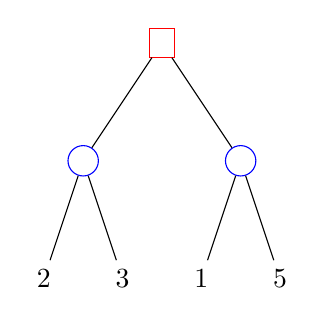
\begin{tikzpicture}%
  [level/.style={sibling distance=20mm/#1}]
  \tikzstyle{box node}=[rectangle,draw=red,inner sep=2]
  \tikzstyle{cir node}=[circle,draw=blue,inner sep=1]
  \node(0)[box node]{\phantom{2}}
  child{node[cir node]{\phantom{2}}
      child{node{$2$}}
      child{node{$3$}}}
    child{node[cir node]{\phantom{1}}
      child{node{$1$}}
      child{node{$5$}}
    };
\end{tikzpicture}
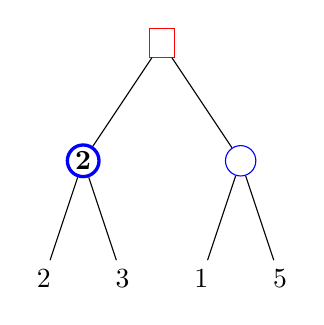
\begin{tikzpicture}%
  [level/.style={sibling distance=20mm/#1}]
  \tikzstyle{box node}=[rectangle,draw=red,inner sep=2]
  \tikzstyle{cir node}=[circle,draw=blue,inner sep=1]
  \node(0)[box node]{\phantom{2}}
    child{node[cir node,very thick]{$\mathbf2$}
      child{node{$2$}}
      child{node{$3$}}}
    child{node[cir node]{\phantom{1}}
      child{node{$1$}}
      child{node{$5$}}
    };
\end{tikzpicture}
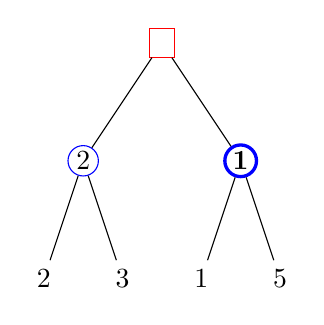
\begin{tikzpicture}%
  [level/.style={sibling distance=20mm/#1}]
  \tikzstyle{box node}=[rectangle,draw=red,inner sep=2]
  \tikzstyle{cir node}=[circle,draw=blue,inner sep=1]
  \node(0)[box node]{\phantom{2}}
    child{node[cir node]{$2$}
      child{node{$2$}}
      child{node{$3$}}}
    child{node[cir node,very thick]{$\mathbf1$}
      child{node{$1$}}
      child{node{$5$}}
    };
\end{tikzpicture}
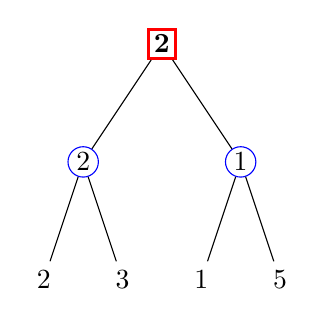
\begin{tikzpicture}%
  [level/.style={sibling distance=20mm/#1}]
  \tikzstyle{box node}=[rectangle,draw=red,inner sep=2]
  \tikzstyle{cir node}=[circle,draw=blue,inner sep=1]
  \node(0)[box node,very thick]{$\mathbf2$}
    child{node[cir node]{$2$}
      child{node{$2$}}
      child{node{$3$}}}
    child{node[cir node]{$1$}
      child{node{$1$}}
      child{node{$5$}}
    };
\end{tikzpicture}
\end{center}

{\scriptsize
\begin{verbatim}
pub fn search_negamax_pruning<Board:GameBoard,Eval:Evaluator<Board>>(b: &mut Board, eval: &eval, ss: &mut SearchStats, depth: isize) -> Board::Scale {
    ss.nodes += 1;
    // check if game is over
    match b.is_terminal() {
        Some(s) => { return s; }
        None => { }
    }
    // check if hit depth bound
    if depth<=0 {
        let e = eval.evaluate(b, ss, depth);
        return Some(e);
    }
    let tomove = b.to_move();
    let other = tomove.other();
    let ml = b.moves();
    // initialize to loss
    let mut best_so_far = Board::Scale::worst(tomove);
    for m in ml {
        b.make_move(m);
        let result = search_negamax_pruning(b, eval, ss, depth - 100);
        b.unmake_move(m);
        best_so_far = Board::Scale::max(tomove, best_so_far, result);
    }
    return best_so_far;
}
\end{verbatim}
}

{\scriptsize
\begin{verbatim}
pub fn search_negamax_ttable<Board:GameBoard,Eval:Evaluator<Board>>(b: &mut Board, eval: &eval, ss: &mut SearchStats, depth: isize) -> Board::Scale {
\end{verbatim}
}

\begin{verbatim}
template <class TMove, bool tt>
result minimax(Board<TMove>& b) {
  hash h;
  if (tt) {
    h = b.Hash();
    if (ttable[h].type == EXACT_BD) {
      ++tthits;
      return ttable[h].res;
    }
  }
  result eval = b.Result();
  ++nodes_searched;
  if (IS_TERMINAL(eval)) {
    if (tt) { ttable[h].res = eval; ttable[h].type = EXACT_BD; }
    return eval;
  }
  result best_v;
  if (b.ToMove() == XX) {
    std::vector<TMove> moves;
    best_v = OO_WIN_IN(-1);
    int num_m = b.Moves(moves);
    for (int m=0; m<num_m; ++m) {
      b.MakeMove(moves[m]);
      result res = minimax<TMove,tt>(b);
      b.UnMakeMove(moves[m]);
      res = PLY_UP_RESULT(res);
      if (res > best_v) best_v = res;
    }
  } else {
    std::vector<TMove> moves;
    best_v = XX_WIN_IN(-1);
    int num_m = b.Moves(moves);
    for (int m=0; m<num_m; ++m) {
      b.MakeMove(moves[m]);
      result res = minimax<TMove,tt>(b);
      b.UnMakeMove(moves[m]);
      res = PLY_UP_RESULT(res);
      if (res < best_v) best_v = res;
    }
  }
  if (tt) { ttable[h].res = best_v; ttable[h].type = EXACT_BD; }
  return best_v;
}
\end{verbatim}

%%%%%%%%%%%%%%%%%%%%
\section{Negamax search}

%%% MOVE THIS TO TICTACTOE DISCUSSION!!!!!

Most real game-playing programs don't use the min-max
formulation for their search, but rather use the so-called
``negamax'' form.  This gives a function which is equivalent
(meaning it will search exactly the same nodes and will
return exactly the same result) but requires less code.
Instead of requiring two different functions (which are nearly identical),
one for the Min player and one for the Max player, negamax search uses
a single search routine which is always trying to maximize the outcome from the
point of view of the player whose turn it is (rather than only player consistently
trying to maximize and the other player trying to minimize).

Another way to think about it is that min-max search uses an absolute
evaluation whereas negamax uses a relative evaluation: evaluating the position
from the point-of-view of the person to move.  The relative evaluation is closer
to how we might actually think about the position if we were playing a game: we
will think that it is good for us or bad for us.  The absolute evaluation is locked
to thinking in terms of a single player.

Generally negamax formulations, though sometimes confusing when first getting into
this area, tend to lead to cleaner and more natural code.  It eliminates a lot of
if-then checks for which side is moving in the search code.  (It can add a
tiny complication to the board evaluation which is often naturally coded in absolute terms.)

\begin{center}
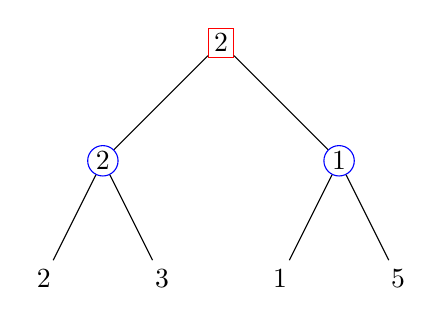
\begin{tikzpicture}%
  [level/.style={sibling distance=30mm/#1}]
  \tikzstyle{box node}=[rectangle,draw=red,inner sep=2]
  \tikzstyle{cir node}=[circle,draw=blue,inner sep=1]
  \node(0)[box node]{$2$}
    child{node[cir node]{$2$}
      child{node{$2$}}
      child{node{$3$}}}
    child{node[cir node]{$1$}
      child{node{$1$}}
      child{node{$5$}}
    };
\end{tikzpicture}
\qquad
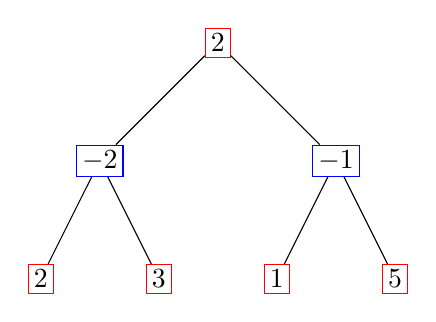
\begin{tikzpicture}%
  [level/.style={sibling distance=30mm/#1}]
  \tikzstyle{box node}=[rectangle,draw=red,inner sep=2]
  \tikzstyle{cir node}=[rectangle,draw=blue,inner sep=2]
  \node(0)[box node]{$2$}
    child{node[cir node]{$-2$}
      child{node[box node]{$2$}}
      child{node[box node]{$3$}}}
    child{node[cir node]{$-1$}
      child{node[box node]{$1$}}
      child{node[box node]{$5$}}
    };
\end{tikzpicture}
\end{center}

%%%%%%%%%%%%%%%%%%%%
\section{Transposition tables}

We can reduce significantly the amount of effort spent in min-max style searching
by recognizing that many positions will arise multiple times in the course of our
search --- for example, one might move a piece twice over the course of two turns, ending up at
the same position, but with a different intermediate step.

%%%%%%%%%%%%%%%%%%%%%%%%%%%%%%%%%%%%%%%%
%%%%%%%%%%%%%%%%%%%%%%%%%%%%%%%%%%%%%%%%
%%%%%%%%%%%%%%%%%%%%%%%%%%%%%%%%%%%%%%%%
%%%%%%%%%%%%%%%%%%%%%%%%%%%%%%%%%%%%%%%%
\part{The Classical Model}


%%%%%%%%%%%%%%%%%%%%%%%%%%%%%%%%%%%%%%%%
%%%%%%%%%%%%%%%%%%%%%%%%%%%%%%%%%%%%%%%%
\chapter{Board representation, move generation}
\label{chap-board-move}

Here 

%%%%%%%%%%%%%%%%%%%%
\section{Array}

The most obvious representation of games set on a grid of cells is to use an array
representation, with each element of the array indicating which piece, if any, in the cell.
This can be a two-dimensional array, matching the layout of the game-board, for example.
Though, it is often more convenient to use a one-dimensional array, with the mapping

Example, chess:
{\scriptsize\begin{verbatim}
    // basic setup
    pub enum Piece { Pawn, Knight, Bishop, Rook, Queen, King };
    pub enum Color { White, Black };
\end{verbatim}}
Matrix or two-dimensional representation:
{\scriptsize\begin{verbatim}
    // definition
    pub struct Board_matrix { cells : [[Option<(Color,Piece)>; 8]; 8], };
    // creation
    let mut b = Board_matrix { cells : [[None; 8]; 8], };
    // put white knight on c2 square
    b.cells[1][2] = Some((Color::White,Piece::Knight));
\end{verbatim}}
{\scriptsize\begin{verbatim}
    // definition
    pub struct Board_array { cells : [Option<(Piece,Color)>; 8 * 8], };
    // creation
    let mut b = Board_array { cells : [None; 8*8], };
    // put white knight on c2 square
    b.cells[1*8 + 2] = Some((Color::White,Piece::Knight));
\end{verbatim}}

%%%%%%%%%%%%%%%%%%%%
\section{Piece lists}

Piece lists are useful for larger games where the the board density
(ratio of number of pieces to squares on the board) is low.  Instead of
directly representing the board, we simply record for each piece, where
it is on the board.  It is often convenient to also represent the board
explicitly, but can still use piece-lists in addition to speed up move generation
or other calculations.

The advantage here is that when doing move generation we don't have to scan the entire board
looking for pieces to move --- we've got the pieces directly accessible and ready to iterate over.
If we organize the lists correctly, we can also get the advantage of generating moves for certain
kinds of pieces before or after other kinds of pieces.

For example, in 5x6 minichess there are 30 squares on the board and the starting position has
20 pieces, for a starting density of $\frac{20}{30} = 0.\bar6$, about~67\%.
On the other hand, in 10x10 amazons, there are 100 squares on the board and there are
only 8 active pieces on the board, with a density of only $\frac{8}{100} = 0.08$, exactly~8\%.
Thus, it would be quite wasteful in amazons for move generation to scan through 100 squares to find the
mere 4 pieces for that side out of the full 100 squares on the board.  Better would be to simply
store directly the locations of the queens for each side in a short list.

%%%%%%%%%%%%%%%%%%%%
\section{0x88}
This is a trick which works for $8\x8$ boards but does not
nicely generalize to other sizes of boards (or to non-rectangular boards).
It is fairly popular in chess playing programs.
The idea is to note that representing a number between 0 and 7 requires exactly 3 bits
and that when generating moves for chess, any putative moves that would take a piece off
of the board would take them to a coordinate which sets the fourth (or ``8'') bit.
Thus, if we represent an x-y coordinate in bits as ``0rrr0ccc'' then we can detect an
illegal coordinate simply by xor'ing with 0x88 = b10001000.

Note that if we then use a grid of cells of size 8x16 = 128, then the valid squares lie on
the ``left hand'' 8x8 grid, so we can use the bit representation as direct index into the array.

For example, using 8-bit integer arithmetic, we have the following, (we mark any invalid squares as **):
\begin{center}\begin{tabular}{c|cccccc}
Square = 0x88 & right 1     & left 1    & down 1      & up 1       & knight (up 2, left 1) \\\hline\hline
$\Delta$      &  +1 = 0x01   &  -1 = 0xFF & -16 = 0xF0  & +16 = 0x10 & +31 = 0x1F            \\\hline
a1 = 0x00     &  b1 = 0x01   &\it ** = 0xFF &\it ** = 0xF0  &  a2 = 0x10 &\it ** = 0x1F            \\
b7 = 0x61     &  c7 = 0x62   &  a7 = 0x60 &  b6 = 0x51  &  b8 = 0x71 &\it ** = 0x80            \\
g2 = 0x16     &  h2 = 0x17   &  f2 = 0x15 &  g1 = 0x06  &  g3 = 0x26 &  f4 = 0x35            \\
h8 = 0x77     &\it ** = 0x78   &  g8 = 0x76 &  h7 = 0x67  &\it ** = 0x87 &\it ** = 0x96            \\
\end{tabular}\end{center}
Notice that all invalid moves end up with an index with highest bit set in one of its two nibbles (4-bit segment).


%%%%%%%%%%%%%%%%%%%%
\section{Mailbox}

%%%%%%%%%%%%%%%%%%%%
\section{Bit-boards}

Bit-boards are a popular approach which are designed to take advantage
of the fact that bit-wise operations are performed in quickly and in parallel
by the computer.  The match of the 64 squares of the chess-board, for example,
match very nicely with the 64 bits in a machine work in a modern 64-bit processor.

The basic idea is that for each piece type, we maintain a vector of bits, one bit
for each square on the board, indicating if there is a piece of that type on the
board.

\subsection{Rotated bit-boards}
\subsection{Kindergarten bit-boards}
\subsection{Magic bit-boards}


%%%%%%%%%%%%%%%%%%%%%%%%%%%%%%%%%%%%%%%%
%%%%%%%%%%%%%%%%%%%%%%%%%%%%%%%%%%%%%%%%
\chapter{Search}
\label{chap-search}

In this chapter we investigate more deeply the issue of searching,

%%%%%%%%%%%%%%%%%%%%
\section{Alpha-beta pruning}
Alpha-beta (\ab) pruning is a way to get the same result
as min-max (or negamax) searching but with significantly reduced amount of search.
The idea is that we we don't really need to search every node, but can ignore significant
parts of the game-tree without affecting the accuracy of our result.

The basic idea is illustrated in the following tree:
\begin{center}
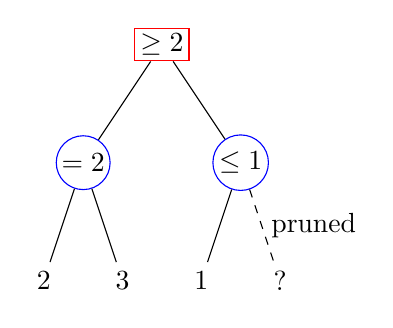
\begin{tikzpicture}%
  [level/.style={sibling distance=20mm/#1}]
  \tikzstyle{box node}=[rectangle,draw=red,inner sep=2]
  \tikzstyle{cir node}=[circle,draw=blue,inner sep=1]
  \node(0)[box node]{$\geq2$}
    child{node[cir node]{$=2$}
      child{node{$2$}}
      child{node{$3$}}}
    child{node[cir node]{$\leq1$}
      child{node{$1$}}
      child{node{?} edge from parent[dashed] node[right]{pruned}}
    };
\end{tikzpicture}
\end{center}
where we can ignore the (subtree off the) final branch by the following reasoning:
the max player can guarantee a result of {\em at least 2} by making the first move, while if
he makes the second move, the min player can ensure a result of {\em no better than 1} by taking
her first move, irrespective of the value of her second move.  Thus the max player would not take
his second move and we do not need to search any further.


The effectiveness of \ab-pruning is extremely sensitive to the order in which we search
the different possibilities at a given node.  The best case is when the first node we search
at each node is the best possible move from that position.  Unfortunately, we typically do not
know the best move (if we know the best move, there would be no need to search in the first
place!)

Worst-case scenario (9 leaf nodes evaluated):
\iffalse
\begin{center}
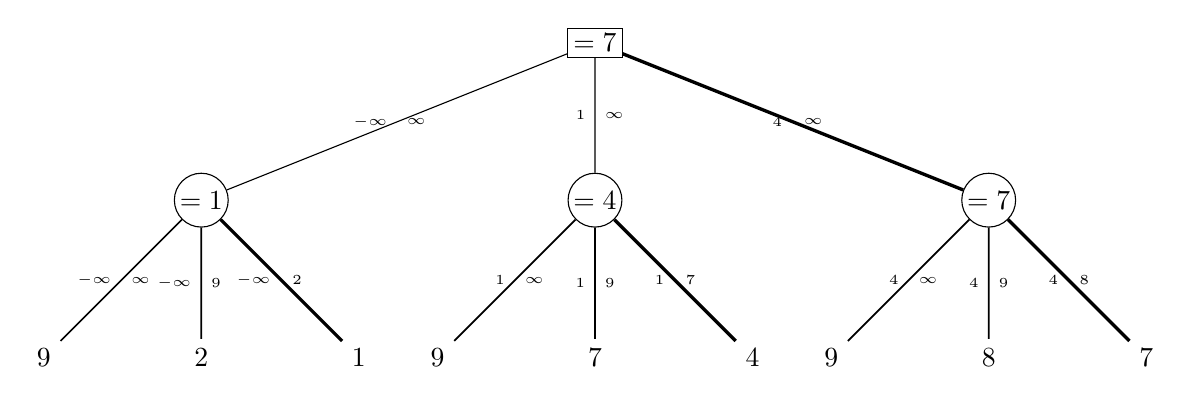
\begin{tikzpicture}%
  %[level/.style={sibling distance=30mm/#1}]
  \tikzstyle{level 1}=[level distance=20mm,sibling distance=50mm]
  \tikzstyle{level 2}=[level distance=20mm,sibling distance=20mm]
  \tikzstyle{maxer}=[rectangle,draw,inner sep=2]
  \tikzstyle{miner}=[circle,draw,inner sep=1]
  \node(0)[maxer]{$=7$}
  child{node[miner]{$=1$}
    child{node{$9$} edge from parent[semithick] node[left]{\tiny$-\infty$} node[right]{\tiny$\infty$}}
    child{node{$2$} edge from parent[semithick] node[left]{\tiny$-\infty$} node[right]{\tiny${9}$}}
    child{node{$1$} edge from parent[very thick] node[left]{\tiny$-\infty$} node[right]{\tiny${2}$}}
    edge from parent node[left]{\tiny$-\infty$} node[right]{\tiny$\infty$}
  }
  child{node[miner]{$=4$}
    child{node{$9$} edge from parent[semithick] node[left]{\tiny$1$} node[right]{\tiny$\infty$}}
    child{node{$7$} edge from parent[semithick] node[left]{\tiny$1$} node[right]{\tiny$9$}}
    child{node{$4$} edge from parent[very thick] node[left]{\tiny$1$} node[right]{\tiny$7$}}
    edge from parent node[left]{\tiny$1$} node[right]{\tiny$\infty$}
  }
  child{node[miner]{$=7$}
    child{node{$9$} edge from parent[semithick] node[left]{\tiny$4$} node[right]{\tiny$\infty$}}
    child{node{$8$} edge from parent[semithick] node[left]{\tiny$4$} node[right]{\tiny$9$}}
    child{node{$7$} edge from parent[very thick] node[left]{\tiny$4$} node[right]{\tiny$8$}}
    edge from parent[very thick] node[left]{\tiny$4$} node[right]{\tiny$\infty$}
  };
\end{tikzpicture}
\end{center}
\fi

Best-case scenario (5 leaf nodes evaluated):
\iffalse
\begin{center}
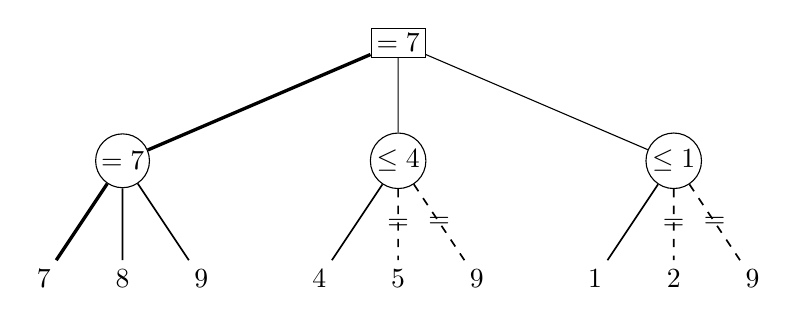
\begin{tikzpicture}%
  %[level/.style={sibling distance=30mm/#1}]
  \tikzstyle{level 1}=[level distance=15mm,sibling distance=35mm]
  \tikzstyle{level 2}=[level distance=15mm,sibling distance=10mm]
  \tikzstyle{maxer}=[rectangle,draw,inner sep=2]
  \tikzstyle{miner}=[circle,draw,inner sep=1]
  \node(0)[maxer]{$=7$}
  child{node[miner]{$=7$}
    child{node{$7$} edge from parent[very thick]}
    child{node{$8$} edge from parent[semithick]}
    child{node{$9$} edge from parent[semithick]}
    edge from parent[very thick]
  }
  child{node[miner]{$\leq4$}
    child{node{$4$} edge from parent[semithick]}
    child{node{$5$} edge from parent[semithick,dashed] node{$=$}}
    child{node{$9$} edge from parent[semithick,dashed] node{$=$}}
  }
  child{node[miner]{$\leq1$}
    child{node{$1$} edge from parent[semithick]}
    child{node{$2$} edge from parent[semithick,dashed] node{$=$}}
    child{node{$9$} edge from parent[semithick,dashed] node{$=$}}
  };
\end{tikzpicture}
\end{center}
\fi

The theoretical improvement we can expect from full width search to optimal \ab-search
was computed by Knuth and [...] which takes a tree with uniform branching
factor $b$ of depth $L$ from $b^L$ nodes for complete search to $b^{\lceil L/2\rceil}+b^{\lfloor L/2\rfloor}$
which translates roughly into allowing us to search to {\em twice} the depth for the same amount of time!

%%%%%%%%%%%%%%%%%%%%
\section{Principal variation}

The {\em principal variant} or {\em PV} is the expected
optimal line of play, where both players are ...

%%%%%%%%%%%%%%%%%%%%
\section{Transposition tables}

Transposition tables are critical for efficient performance.

A crucial element of using transposition tables is the hash function --- the
function which takes a position and 

\subsection{Zobrist hashing}
The standard approach to hashing was ... by Zobrist in ...
It is a clever approach which applies easily to many different games
and implementation styles.

The core idea is to assign a (pseudo-)random number to each individual color, piece, and square
combination.  For example, in chess, we'll have a number (code) for white knight at a1, white knight at a2,
..., black rook at h8.  Then, to compute the hash of a position, we simply take the ``exclusive or''
(or ``xor'' or $\oplus$) of this code for each piece on the board.
\footnote{
  The xor of individual bits is defined by $0\oplus1=1\oplus0=1$ and $0\oplus0=1\oplus1=0$.
  The xor of two $n$-bit integers is simply the bit-by-bit xor of the individual bits in the
  integer representations.  You may check that, for example, $1\oplus3=2$ and $1\oplus4=5$.
}

Now, the xor operator has the beautiful property that $(a\oplus b)\oplus b = a$ for any $a$ and $b$.
In other words, if I take a number and xor any other number with it twice, I end up with my original number.
Additionally, xor operates bit-by-bit on an integer, so it is a very fast operation to execute by the CPU.

\subsection{BCH hashing}

%%%%%%%%%%%%%%%%%%%%
\section{Iterative deepening}

In iterative-deepening, we do a series of searches to increasing depth, rather than
deciding beforehand a fixed depth to search

As we will see later, using iterative deepening makes for good use of
time --- allowing us to do the best search we can in a given time interval,
even though ...

Although re-searching the same position multiple times may seem like a ridiculous waste
of time, it is actually quite efficient and it is possible for an iterative-deepened search to
a given depth to actually take {\em less} time than a single search directly to that depth!
The main reason for this is that with the use of a transposition table, we are able to use
the results of shallower searches to sort the moves when doing a deeper search, thus generally
achieving better results for \ab-pruning.  Another point to note is that often shallower search results
stored in the transposition table are re-used in the deeper search allowing for savings in the
deeper search; that is, sub-trees can often be reached via different move sequences of different lengths.

%%%%%%%%%%%%%%%%%%%%
\section{Quiescence search}

The idea behind quiescence search is to end search lines only at ``quiet'' positions.
This stabilizes evalations and helps to avoid the so-called ``horizon effect''.
It will also add to the tactical strength.

As an example of the horizon effect, consider the following chess position:
\[ ... \]
If we use a standard fixed-depth alpha-beta search we get the following lines ...
notice that it isn't until we reach a search depth of ... that the search finally
realizes that snagging the pawn isn't safe.
On the other hand using quiescence extensions we get ...

The definition of quiet or quiescent position depends on the game and the nature
of the search can vary.

For \g{chess}, a common approach to quiescence search is
to search all captures, checks,
and check responses.  Note that it is important to allow a ``stand pat'' option also when
searching (where a side can just accept the static evaluation instead of following
further in the quiescence search.

Following captures is a relatively safe and for many games, is a self-limiting approach,
since each capture can reduce the number of pieces on the board.  However, this is not
universally true.
For example, in \g{shogi}, doing a quiescence search which searched captures as well as drops would
lead to horrendous search explosions as capture-drop sequences can be unending
(with each captured piece being reused as a possible drop by the capturing side.)

%%%%%%%%%%%%%%%%%%%%
\section{Null-move pruning}
Null-move pruning is a forward-pruning technique based on the assumption that it
is always better to make a move than to ``pass''.
It can significantly reduce the number of nodes searched with a minor reduction
in the strength (due to the occasional ...)

\subsection{Adaptive null-move pruning}
For chess it was ...
$R=3$ was somewhat over-aggressive in pruning,
while $R=2$ is

\subsection{Verified null-move pruning}

%%%%%%%%%%%%%%%%%%%%
\section{Other heuristics}
Here we cover some heuristic pruning techniques which are ``unsound'' --- unlike
\ab-pruning, they are not guaranteed to return the exact min-max value.  However,
in practice they are extremely effective.
\subsection{Killer moves}
\subsection{History heuristic}
\subsection{Razoring}
\subsection{Futility pruning}
\subsubsection{Extended futility pruning}
\subsection{Search extensions}

%%%%%%%%%%%%%%%%%%%%%%%%%%%%%%%%%%%%%%%%
%%%%%%%%%%%%%%%%%%%%%%%%%%%%%%%%%%%%%%%%
\chapter{Evaluation}
\label{chap-evaluation}

In this chapter we discuss the evaluation of

%%%%%%%%%%%%%%%%%%%%
\section{Material}
The most significant of components for evaluation
of positions for most chess-like games is material:
the positions ...

%%%%%%%%%%%%%%%%%%%%
\section{Piece-square bonus}
It is known that in \g{chess}, for example, it is generally
advantageous for knights to occupy central squares and that
usually it is bad to have a knight in a corner square.  This
can be generalized to giving a bonus or malus for each piece
being in any particular position on the board.

Similarly, certain general tactics can be ``encouraged'' by
giving bonuses and maluses:
\begin{itemize}
  \item General piece centralization
  \item Pawn pushing towards promotion squares
  \item Bishops on long diagonals (fianchetto)
  \item ...
\end{itemize}


%%%%%%%%%%%%%%%%%%%%
\section{Mobility}

Mobility describes the available moves by each side.  The simplest
approach would simply count the possible moves in the given position.
More sophisticated measures include counting attacks differently
than simple moves, ``x-ray'' moves (moves or attacks which are blocked by
one's own pieces but which ...
TODO...

%%%%%%%%%%%%%%%%%%%%
\section{Structure, Shape}

For games such as \g{chess} or \g{sh\=ogi},
we have ``static'' features of the
position --- features of the position which tend to persist over longer
stretches of the game, features which involve the interaction of many pieces,
...

For \g{chess}, this would include pawn-structure (e.g. isolated
pawns, double pawns, passed pawns, protected passed pawns, etc.) whereas

For \g{shogi} we have ``shape'' TODO...

%%%%%%%%%%%%%%%%%%%%
\section{Square-control bonus}

%%%%%%%%%%%%%%%%%%%%
\section{Hanging pieces, defended pieces}

\subsection{SEE}
\subsection{SOMA}
\subsection{SUPER-SOMA}

%%%%%%%%%%%%%%%%%%%%%%%%%%%%%%%%%%%%%%%%
%%%%%%%%%%%%%%%%%%%%%%%%%%%%%%%%%%%%%%%%
%%%%%%%%%%%%%%%%%%%%%%%%%%%%%%%%%%%%%%%%
%%%%%%%%%%%%%%%%%%%%%%%%%%%%%%%%%%%%%%%%
\part{The Monte Carlo Revolution}

%%%%%%%%%%%%%%%%%%%%%%%%%%%%%%%%%%%%%%%%
%%%%%%%%%%%%%%%%%%%%%%%%%%%%%%%%%%%%%%%%
\chapter{MCTS}
\label{chap-mcts}

Monte-carlo tree search (MCTS) is a relatively new approach to solving
games that has become extremely effective at certain kinds of games, such
as \g{go}, where traditional \ab-approaches have difficulties, both
due to the high branching factor and to the challenge of constructing a good
evaluation function.

%%%%%%%%%%%%%%%%%%%%
\section{UCB}


%%%%%%%%%%%%%%%%%%%%%%%%%%%%%%%%%%%%%%%%
%%%%%%%%%%%%%%%%%%%%%%%%%%%%%%%%%%%%%%%%
\chapter{Extensions}
\label{chap-mcts-extensions}

%%%%%%%%%%%%%%%%%%%%
\section{AMAF}

%%%%%%%%%%%%%%%%%%%%
\section{RAVE}

%%%%%%%%%%%%%%%%%%%%
\section{Incorporating domain knowledge}



%%%%%%%%%%%%%%%%%%%%%%%%%%%%%%%%%%%%%%%%
%%%%%%%%%%%%%%%%%%%%%%%%%%%%%%%%%%%%%%%%
%%%%%%%%%%%%%%%%%%%%%%%%%%%%%%%%%%%%%%%%
%%%%%%%%%%%%%%%%%%%%%%%%%%%%%%%%%%%%%%%%
\part{Other}

%%%%%%%%%%%%%%%%%%%%%%%%%%%%%%%%%%%%%%%%
%%%%%%%%%%%%%%%%%%%%%%%%%%%%%%%%%%%%%%%%
\chapter{UI}
\label{chap-ui}

In this chapter we 

%%%%%%%%%%%%%%%%%%%%
\section{GGS}
%%%%%%%%%%%%%%%%%%%%
\section{UCI}
%%%%%%%%%%%%%%%%%%%%
\section{UGI}
%%%%%%%%%%%%%%%%%%%%
\section{UGE}
%%%%%%%%%%%%%%%%%%%%
\section{XBoard}
%%%%%%%%%%%%%%%%%%%%
\section{Fritz}

%%%%%%%%%%%%%%%%%%%%%%%%%%%%%%%%%%%%%%%%
%%%%%%%%%%%%%%%%%%%%%%%%%%%%%%%%%%%%%%%%
\chapter{Time management}
\label{chap-time}

In this chapter we 

%%%%%%%%%%%%%%%%%%%%
\section{Time controls}
There are many different time-controls that exists for different games.
For example, there may be a fixed amount of time for each side for all moves
made in the game, or there may be a set amount of time for each move made (where
the unused time may be accumulated for later (with a possible cap) or may simply
be lost.)

\begin{itemize}
\item Chess: In chess, there are a variety of popular time-controls.
\item Go:
\item Arimaa: from {\tt http://arimaa.com/arimaa/learn/matchRules.html}
and where the 2011 Arimaa Open Classic and World Championship
is being played to {\tt 60s/5m/75/0/4h/4m} for the Swiss preliminary and
{\tt 90s/5m/75/0/6h/5m} for the FDE final.

The time specification {\tt 60s/5m/75/0/4h/4m} means, for example,
  \begin{itemize}
  \item 60 seconds per move
  \item 5 minutes in the starting reserve
  \item 75\% of remaining move time gets added to reserve
  \item 4 hours maximum limit for the game
  \item 4 minutes maximum turn time 
  \end{itemize}
In other words:
On each turn a player gets 60 seconds per move.
If a move is not completed in this time then the reserve time may be used.
There is a starting reserve of 5 minutes.
If the reserve time is used up and the player has still not made a move then the player will lose on time.
If the move is made in less than 60 seconds then 75\% of the remaining move time is added to the reserve.
A players turn may not exceed more than 4 minutes regardless of how much time is in reserve.
If the game is not completed within 4 hours, it will be stopped and the winner determined by score.
\item Computer Olympiad: in the ICGA Computer Olympiads, the most common time control is ...
\end{itemize}

\subsection{Arimaa Time Controls Specification}
The time control used for Arimaa is given by a 6-part specification {\tt M/R/P/L/G/T} where
\begin{itemize}
\item {\tt M} is the number of minutes:seconds per move; required
\item {\tt R} is the number of minutes:seconds in reserve; required
\item {\tt P} is the percent of unused move time that gets
            added to the reserve; optional defaults to 100
\item {\tt L} is the number of minutes:seconds to limit the reserve;
            0 means no limit; optional; defaults to 0
\item {\tt G} is the number of hours:minutes after which time
            the game is halted and the winner is determined
            by score. {\tt G} can also be specified as the maximum
            number of moves by ending with 't'; 0 means no
            limit; optional; defaults to 0
\item {\tt T} is the number of minutes:seconds within which
            a player must make the move; 0 means no limit;
            optional; defaults to 0
\end{itemize}
Different time units for any of the time control fields
can be specifed by adding one of the following letters
after the numbers.  In such cases the letter serves as
the separator and {\tt :} should not be used.
\begin{itemize}
\item {\tt s} - seconds
\item {\tt m} - minutes
\item {\tt h} - hours
\item {\tt d} - days
\end{itemize}
For example:  {\tt 24h5m10s/0/0/0/60d} means 24 hours, 5 minutes
and 10 seconds per move and the game must end after 60 days.
Such a time control may be used in a postal type match.
\begin{itemize}
\item
The game time parameter ({\tt G}) can also be specified in terms
  of maximum number of turns each player can make by adding
  the letter {\tt t} after the number.
\item
On each turn a player gets a fixed amount of time per 
  move (M) and there may be some amount of time left 
  in the reserve (R).
\item
If a player does not complete the move within the move
  time (M) then the time in reserve (R) is used.  If there is
  no more time remaining in reserve and the player has
  not completed the move then the player automatically loses.
  Even if there is time left in the move or reserve, but the player
  has not made the move within the maximum time allowed
  for moves (T) then the player automatically loses.
\item
If a player completes the move in less than the
  time allowed for the move (M), then a percentage (P) of the 
  remaining time is added to the players reserve.   The 
  result is rounded to the nearest second.  This parameter
  is optional and if not specified, it is assumed to be 100\%.
\item
An upper limit (L) can be given for the reserve so that 
  the reserve does not exceed L when more time is added to 
  the reserve.  If the initial reserve already exceeds this
  limit then more time is not added to the reserve until it
  falls below this limit. The upper limit for the reserve is 
  optional and if not given or set to 0 then it implies that 
  there is no limit on how much time can be added to the reserve.
\item
For practical reasons a total game time (G) may be
  set.  If the game is not finished within this allotted time
  then the game is halted and the winner is determined by 
  scoring the game.  This parameter is optional and if
  not given (or set to 0) it means there is no limit on the 
  game time. Also instead of an upper limit for the total
  game time, an upper limit for the total number of turns each
  player can make may be specified by adding the letter 't'
  after the number. After both players have taken this many 
  turns and the game is not finished the winner is determined 
  by scoring the game.
\item
For games which use a time per move of less than 1 minute,
  both players are always given 1 minute of time to setup the
  initial position in the first move of the game.  If the setup
  is not completed in 1 minute then the reserve time (R) is also used.
  The unused time from the setup move is not added to the
  reserve time.
\end{itemize}
Some examples:
\begin{itemize}
\item Example 1: {\tt 0/5} means 0 minutes per move with 5 minutes
  in reserve (per player). This is equivalent to G/5 in Chess; it
  means each player has a total of 5 minutes of time
  to play.  If a player runs out of time before the
  game is over, the player loses.  This is known as
  Blitz or "Sudden Death" time control in Chess.

\item Example 2: {\tt 0:12/5} means 12 seconds per move
  with 5 minutes in reserve and all of the unused time from
  each move is added to the reserve time.  It is similar 
  to "5 12" in Chess which means "Game in 5 minutes with 
  a 12 second increment".  After each move 12 seconds is 
  added to the remaining time. This is known as Incremental 
  time control in Chess.

\item Example 3: {\tt 3/0} means 3 minute per
  move and no reserve time, but 100 percent of the
  unused time for each move is added to the reserve.  This
  guarantees that each player will make at least 40 moves 
  in 2 hours.  This is similar 
  to the "40/2" Quota System time control used in Chess.
  
\item Example 4: {\tt 0:30/5/100/3} means 30 seconds per move
  with 5 minutes in reserve and 100\% of the unused time from
  each move is added to the reserve time.  When the reserve 
  already exceeds the limit, more time is not added to it.  
  When the reserve falls below 3 minutes more time can be 
  added to it, but the reserve is capped at 3 minutes.
\item   Example 5: {\tt 4/2/50/10/6}
    This means 4 minutes per move with a starting reserve
    of 2 minutes.  After the move 50\% of the time remaining
    for the move (rounded to the nearest second) is added 
    to the reserve such that it does not exceed 10 minutes.  
    There is a limit of 6 hours for the game after which time 
    the game is halted and the winner is determined by score.  
\item   Example 6: {\tt 4/4/100/4/6}
    This means 4 minutes per move and a starting
    reserve of 4 minutess. 100\% percent of the unused move
    time gets added to the reserve such that it does not exceed 
    4 minutes.  There is a time limit of 6 hour for the game
    after which the winner is determined by score.
\item   Example 7: {\tt 4/4/100/4/90t}
    This is the same as above, but the game ends after both
    players have made 90 moves. Thus it ends after move 90
    of silver is completed.
\item   Example 8: {\tt 4/4/100/4/90t/5}
    This is the same as above, but the players may not take
    more than 5 minutes for each turn even if there is 
    still time remaining in reserve.
\end{itemize}


%%%%%%%%%%%%%%%%%%%%
\section{Estimation of remaining time}
%%%%%%%%%%%%%%%%%%%%
\section{Control}
%%%%%%%%%%%%%%%%%%%%
\section{Pondering}
{\em Pondering} is where the computer uses the time during the opponent's move to
think.

The standard approach is to assume that the opponent will make the move given as the
response in the principal variation (PV) and to start ``thinking'' based on this assumption.
As long as this correctly predicts the move 50\% or more it will pay off well.  (If the
opponent makes a different move, we have to restart the search and the effort is lost.)

%%%%%%%%%%%%%%%%%%%%
\section{Example: Crafty}

Here we describe the method for time-control used in Crafty (version xx.xxx).

%%%%%%%%%%%%%%%%%%%%
\section{Example: Gerbil}

The open-source chess engine Gerbil supports a basic sudden-death time-control
with or without an increment; a fixed time per move;
and moves-per-period time-control.

It has variables \verb|base| and \verb|extra| in the engine.

For a fixed time $t$ per move, it is quite simple: use all the given
time $\verb|base|=t$ and there is no extra time $\verb|extra|=0$.

For sudden-death with no increment, it uses 

{\scriptsize
\begin{verbatim}
    case tctINCREMENT:
        if (pcon->tc.tmIncr) {
            TM    tmTarget;

            //    An increment time control tries not to go below the increment
            //    plus 30 seconds, or 6 times the increment, whichever is more.
            //
            //    If it finds itself below that, it will the increment minus
            //    1/10 of the time by which it is under the target.
            //
            //    If it is over that, it will use the increment plus 1/20 of
            //    the time by which it is over the target.
            //
            //    So the program will drift slowly down to the target, but if
            //    it gets a ways below it, it will tend to come up quickly.
            //
            //    There are a zillion different increment time controls, and
            //    sometimes I could end up with a stupid base time.  I try hard
            //    to make sure the base time doesn't go below zero, which would
            //    be very bad since my time quantity is an unsigned value.
            //
            //    I will try hard to use >= half of the increment.  I will also
            //    make sure to not use more than half the remaining time (which
            //    is taken care of by the code at "lblSet".
            //
            tmTarget = pcon->tc.tmIncr + 30000;
            if (tmTarget < 6 * pcon->tc.tmIncr)
                tmTarget = 6 * pcon->tc.tmIncr;
            if (pcon->ss.tmUs >= tmTarget)
                tmBase = pcon->tc.tmIncr + (pcon->ss.tmUs - tmTarget) / 20;
            else    // The following statement can go negative on an unsigned.
                tmBase = pcon->tc.tmIncr - (tmTarget - pcon->ss.tmUs) / 10;
            Assert(sizeof(long) == sizeof(TM));
            if ((long)tmBase < (long)pcon->tc.tmIncr / 2)
                tmBase = pcon->tc.tmIncr / 2;
        } else {
            //
            //    A zero-increment time control will use 1/30 of the remaining
            //    time down to 10 minutes, 1/40 down to one minute, and 1/60
            //    after that.
            //
            if (pcon->ss.tmUs >= 600000)        // 10 minutes.
                tmBase = pcon->ss.tmUs / 30;
            else if (pcon->ss.tmUs > 60000)    // 1 minute.
                tmBase = pcon->ss.tmUs / 40;
            else
                tmBase = pcon->ss.tmUs / 60;
        }
        //    This code dummy-checks "tmBase", assigns "tmExtra", then assigns
        //    an end-time based upon "pcon->ss.tmStart".
        //
        //    First I check to see if I'm scheduled to eat more than half of
        //    my remaining time.  I put a ceiling at that amount, right off.
        //
        //    Next, I'll assign some emergency time.  This is 3x the base time,
        //    with a ceiling on base + extra of 1/2 the remaining time.  I will
        //    also allocate no emergency time if I have < 30 seconds on the
        //    clock.
        //
        //    So there will be plenty of "extra" time if there is time left,
        //    otherwise there is little or none.
        //
lblSet:    if (tmBase > pcon->ss.tmUs / 2)
            tmBase = pcon->ss.tmUs / 2;
        tmExtra = (pcon->ss.tmUs < 20000) ? 0 : tmBase * 3;
        if (tmBase + tmExtra > pcon->ss.tmUs / 2)
            tmExtra = pcon->ss.tmUs / 2 - tmBase;
        pcon->ss.tmEnd = pcon->ss.tmStart + tmBase;
        pcon->ss.tmExtra = tmExtra;
        break;
    case tctFIXED_TIME:
        tmBase = pcon->tc.tmBase;        // Use *all* the time.
        pcon->ss.tmEnd = pcon->ss.tmStart + tmBase;
        pcon->ss.tmExtra = 0;            // No emergency time.
        break;
    case tctTOURNEY:
        movMade = pcon->gc.ccm / 2 + pcon->gc.movStart - 1;
        while (movMade >= pcon->tc.cMoves)
            movMade -= pcon->tc.cMoves;
        movLeft = pcon->tc.cMoves - movMade;
        Assert(movLeft >= 1);
        //
        //    This expression is kind of nasty.  It is:
        //
        //        Time / (3/4 x Moves + 3)
        //
        //    The point of the "3" is to make sure there's some extra time pad
        //    at the beginning, and the point of the 3/4 is to make sure that
        //    earlier moves take a little longer per move.
        //
        //    This expression has been reduced to ...
        //
        //        (4 * Time) / (3 * Moves + 12)
        //
        //    .. by multiplying the top and the bottom by 4.  This helps out
        //    with the integer math.
        //
        tmBase = (4 * pcon->ss.tmUs) / (3 * movLeft + 12);
        goto lblSet;
    }
\end{verbatim}
}

{\scriptsize
\begin{verbatim}
//    This is called a whole bunch of times via the engine/interface protocol.
//    Given what is known about the time control, the current time, and the
//    search depth, this may set "ptcon->fTimeout", which will eventually finish
//    the search.

//    This routine has a built-in defense against cases where someone might try
//    to force a move before the first ply has been fully considered.  It will
//    simply ignore such cases.

void VCheckTime(PCON pcon)
{
    TM    tmNow;

    if (pcon->ss.plyDepth == 1)    // Can't time out before a one-ply
        return;                    //  search is finished.
    if (pcon->smode != smodeTHINK)
        return;
    if ((tmNow = TmNow()) >= pcon->ss.tmEnd) {
        //
        //    Time has expired.  Check for a fail-high or fail low and try to
        //    add some time.  Don't add any time if we're already dead lost and
        //    just slowly collapsing, or if we are won and are probably failing
        //    high repeatedly.  The standard for "won" is a little greater than
        //    for "lost".
        //
        if ((pcon->ss.prsa != prsaNORMAL) && (pcon->ss.val < valROOK) &&
            (pcon->ss.val >= -valMINOR))
            if (pcon->ss.tmExtra < 1000) {
                pcon->ss.tmEnd += pcon->ss.tmExtra;
                pcon->ss.tmExtra = 0;
            } else {
                pcon->ss.tmEnd += pcon->ss.tmExtra / 2;
                pcon->ss.tmExtra -= pcon->ss.tmExtra / 2;
            }
        if (tmNow >= pcon->ss.tmEnd)
            pcon->fTimeout = fTRUE;
    }
}
\end{verbatim}
}


%%%%%%%%%%%%%%%%%%%%
\section{Example: Glaurung}

As an interesting case-study, we examine the logic used by the open-source
chess engine Glaurung.  (From examining the source code.)

The basic timing method involves three variables to control the time
spent on a search:
\verb|max_time| --- the target time to spend on the search,
\verb|extra_time| --- a possible amount of extra time to search in certain
cases, and \verb|absolute_max_time| --- an absolute maximum, which will abort
the search when exceeded.
It supports sudden-death (with or without increment) or
moves-per-period time-controls.

For sudden-death time-control with $t$ remaining time (in milliseconds)
and no increment, it sets:
\begin{eqnarray*}
\verb|max_time| &=& t/40 \\
\verb|absolute_max_time| &=& t/8
\end{eqnarray*}
If there is an increment of $i$ milliseconds, then it uses
\begin{eqnarray*}
\verb|max_time| &=& t/30+i \\
\verb|absolute_max_time| &=& \max(t/4,i-100)
\end{eqnarray*}
For moves-per-period style of time-control, it sets
\begin{eqnarray*}
\verb|max_time| &=& t/\min(\verb|moves_to_go|,20) \\
\verb|absolute_max_time| &=& \min(4t/\verb|moves_to_go|, t/3)
\end{eqnarray*}
unless there is only a single move left to go in which case it uses
\begin{eqnarray*}
\verb|max_time| &=& t/2 \\
\verb|absolute_max_time| &=& \min(t/2,t-500)
\end{eqnarray*}

Glaurung uses an iterative-deepening search strategy, and for
the first 5 iterations, it sets $\verb|extra_time|$ to zero,
otherwise (for the 6th and higher iterations) if the best move has changed
in the last two iterations it will set
\[ \verb|extra_time|
  = {\verb|bmcc|}_{\text{it}}\x(\verb|max_time|/3)
  + {\verb|bmcc|}_{\text{it}-1}\x(\verb|max_time|/6) \]
where ${\verb|bmcc|}_{\text{it}}$ is the "best-move change-count" --- the number
of times that the best move has changed in the $\text{it}$'th iteration.

Glaurung will stop a search early if there seems to be an ``easy'' move (a move
which is clearly better than the rest).  If it has done at least 5 iterations
and:
{\scriptsize
\begin{verbatim}
    // Stop search early if one move seems much better than the rest:
    if(RSI->iteration >= 5 && RSI->easymove &&
       ((RSI->root_moves.moves[0].cumulative_nodes > (RSI->nodes*85)/100 &&
         get_time() - RSI->start_time > RSI->max_time/16) ||
        (RSI->root_moves.moves[0].cumulative_nodes > (RSI->nodes*99)/100 && 
         get_time()-RSI->start_time > RSI->max_time/32)) &&
       !RSI->infinite && RSI->thinking_status!=PONDERING) {
      break;
    }
\end{verbatim}
}

The search will be ended if most of \verb|max_time| has been used at the end
of an iteration (because there wouldn't be time to complete the next iteration
in any case.)  Specifically if the time used so far exceeds
$(\verb|max_time| + \verb|extra_time|)\x80/128$.

During the search, the timeout is
{\scriptsize
\begin{verbatim}
void check_for_timeout(void) {
  int t;
  static int last_info_time;

  t = get_time() - RSI->start_time;
  if(t < 1000) last_info_time = 0;
  else if(t - last_info_time >= 1000) {
    mutex_lock(IOLock);
    printf("info nodes " llu_format " nps " llu_format " time %d hashfull %d\n",
           RSI->nodes, (RSI->nodes*1000ULL)/((uint64) t), t, hashfull());
    mutex_unlock(IOLock);
    last_info_time = t;
    if(Options->currline) Threads[0].print_currline = true;
  }
  if(RSI->thinking_status != PONDERING && RSI->iteration >= 2 &&
     ((!RSI->infinite && 
       (t > RSI->absolute_max_time
        || (RSI->root_moves.current == 1 && t > RSI->max_time+RSI->extra_time) 
        || (!RSI->fail_high && t > 6 * (RSI->max_time+RSI->extra_time)))) ||
      (RSI->node_limit && RSI->nodes >= RSI->node_limit) ||
      (RSI->exact_time && t >= RSI->exact_time)))
    RSI->thinking_status = ABORTED;
}
\end{verbatim}
}


%%%%%%%%%%%%%%%%%%%%%%%%%%%%%%%%%%%%%%%%
%%%%%%%%%%%%%%%%%%%%%%%%%%%%%%%%%%%%%%%%
\chapter{Advanced Search}
\label{chap-advanced-search}

In this chapter we investigate more deeply the issue of searching,

%%%%%%%%%%%%%%%%%%%%
\section{Trappy min-max}

This is a game-independent method described in~\cite{gordonreda}
for automatically playing in a way to set traps for the opponent
--- based on the idea that if you search more deeply than your opponent you can
identify misleading lines of play (when the best-move to play at a shallower
search depth is given a much lower evaluation at a deeper search depth).
You may then choose a non-optimal move as long as it is not too much worse than the
best move, but for which the obvious reply by the opponent is actually much worse ...TODO...

This kind of approach is best used against ``fallible'' opponents (human players, for example)
or by brute-force deep-search based programs against shallower searching ... blah ...

%%%%%%%%%%%%%%%%%%%%
\section{Negascout}
%%%%%%%%%%%%%%%%%%%%
\section{Null-window search}
%%%%%%%%%%%%%%%%%%%%
\section{Aspiration search}
%%%%%%%%%%%%%%%%%%%%
\section{PVS}
%%%%%%%%%%%%%%%%%%%%
\section{MTD(f)}

%%%%%%%%%%%%%%%%%%%%
\section{Conspiracy number}
Conspiracy number search is a best-first search method.
It is based on the idea of searching to a given level of confidence, measured
in the number of nodes we've evaluated which would need to ``conspire'' in being
wrongly evaluated in order to change our evaluation of the root.  (We may also think
of this as a measure of robustness --- how many nodes could be systematically mis-evaluated
without affecting our result.)

If we have a search tree, there will be a certain
number of ``leaf'' nodes that we have reached in our search.  (That is,
nodes where we use the evaluation function to get an evaluation of the position.)
Define the conspiracy number of {\em any} node in the tree to be the minimum number
of {\em leaf} nodes that would need to change their value in order to
change the value of that given node.  In fact, for different evaluation values, there
may be different numbers ... blah blah....

Standard example repeated {\it ad nauseum}:
\begin{center}
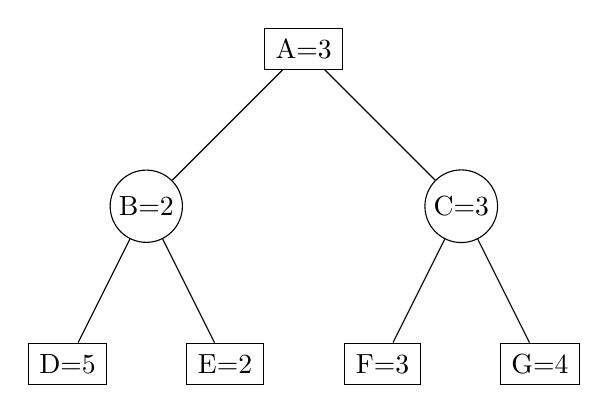
\begin{tikzpicture}%
  %[level/.style={sibling distance=40mm/#1}]
  \tikzstyle{level 1}=[level distance=20mm,sibling distance=40mm]
  \tikzstyle{level 2}=[level distance=20mm,sibling distance=20mm]
  \tikzstyle{boxn}=[rectangle,draw,inner sep=4]
  \tikzstyle{cirn}=[circle,draw,inner sep=2]
  \node(0)[boxn]{A=3}
  child{node[cirn]{B=2}
    child{node[boxn]{D=5}}
    child{node[boxn]{E=2}}}
  child{node[cirn]{C=3}
    child{node[boxn]{F=3}}
    child{node[boxn]{G=4}}}
    ;
\end{tikzpicture}
\\\noindent
where for node A we have
\\\noindent
\begin{tabular}{ccc}
  value & cn & nodes which have to change \\
  1 & 2 & (D or E) and (F or G) \\
  2 & 1 & F or G \\
  3 & 0 & - \\
  4 & 1 & E or F \\
  5 & 1 & E \\
  6 & 2 & (D and E) or (F and G)
\end{tabular}
\end{center}

\subsection{Alpha-beta conspiracy search}

In \cite{alphabetaconspiracy}, McAllester and Yuret describe a variant of \ab-search
which is derived from conspiracy number search but is a depth-first rather than best-first search
as in the original conspiracy numbers algorithm.

The idea incorporates two ``depth'' numbers $d_{\max}$ and $d_{\min}$ instead of a single one as in
standard \ab-search.  It also includes an additional list of lists of static values of siblings of
a given node and its ancestors.

We also define a number \verb|delta|, the ``singular margin'', as well as a real-valued, increasing function
$S(k)$ such that $S(0)=0$ and $\lim_{k\to\infty}S(k)=1$ and which gets close to 1 before the typical
branching factor $b$.  (For example, we might take
\[ S(k) = \begin{cases}1&\text{if $k\geq b$}\\1-\left(\frac{b-k}{b}\right)^\gamma&\text{otherwise}\end{cases}\]
where $b$ is the typical branching factor of the game we are analyzing.
The parameter $\gamma$ can be tuned from 1 to $b$ to move continuously from conspiracy depth to classical
ply depth.)

To start the search, one calls
{\scriptsize
\begin{verbatim}
  ABC(root, -infinity, +infinity, d_max, d_min, [], [])
\end{verbatim}
}
where
{\scriptsize
\begin{verbatim}
  ABC(node, alpha, beta, d_max, d_min, max_options, min_options) {
    if (terminate?(node, alpha, beta, d_max, d_min, max_options, min_options)) {
      return the static value of node;
    }
    if (node is a max-node) {
      v := alpha;
      for each child c of node {
        sib_options = list of static values of siblings of c;
        next_max_options = [sib_options] ++ max_options;
        v = max(v, ABC(c, v, beta, d_max, d_min, next_max_options, min_options));
        if (v >= beta) { return v; }
      }
      return v;
    } else {
      ... dual of the max-node case ...
    }
  }
\end{verbatim}
}
and
{\scriptsize
\begin{verbatim}
  terminate?(node, alpha, beta, d_max, d_min, max_options, min_options) {
    v = static value of node;
    if ((v >= beta) && (max_depth(beta, max_options) >= d_max)) {
      return true;
    }
    if ((v <= alpha) && (min_depth(alpha, min_options) >= d_min)) {
      return true;
    }
    if ((alpha < v < beta) && (max_depth(v, max_options) >= d_max) && (min_depth(v, min_options) >= d_min)) {
      return true;
    }
    return false;
  }
\end{verbatim}
}
and
{\scriptsize
\begin{verbatim}
  max_depth(v, max_options) {
    return sum over all value lists L in max-options of S(k)
      where k is the number of elements of L > v-delta
  }
\end{verbatim}
}
and
{\scriptsize
\begin{verbatim}
  min_depth(v, min_options) {
    return sum over all value lists L in min-options of S(k)
      where k is the number of elements of L < v+delta
  }
\end{verbatim}
}

%%%%%%%%%%%%%%%%%%%%
\section{Proof number}

%%%
Implementation idea: to reduce space, assume pre-computed max number of nodes to search.  Then we can 
pre-allocate huge array of elements.  Children of node are allocated in adjacent sweep of elements from
array - so parent just needs index of first child (and number of children).  Note that this doesn't work
well with strategies that free nodes etc.
%%%

Proof number search is a best-first search method which, as the name suggests, attempts
to ``prove'' a result for a position.  It does not rely on an evaluation function {\it per se},
but rather on a binary proposition or goal, for example, "Win for white" or "Not a loss for black".
One can also imagine other propositions such as "White wins a queen".
The search process then attempts to prove or disprove the proposition.
In the discussion below, we will simply assume that the goal is "Win" for the max player for
ease of exposition.

The {\it proof number}\index{proof number} of a node is the number of nodes below it that need to
be shown to be wins for the node itself to be a win and the {\it disproof number}\index{disproof number}
is the number of its descendents that need to be proved losses for the node to be a loss.
For a non-terminal leaf-node, we set both the proof and disproof numbers to 1.
Thus, for a terminal node which is a win, we have a proof number of zero~($0$) and a disproof number of infinity~($\infty$).
Similarly, for a terminal node which is a loss, the proof number is~$\infty$ and the disproof number is~$0$.
For internal nodes, we can compute inductively their (dis)proof numbers: if a node $X$ is a Max node,
then the proof number $X.p$ and disproof number are given by
\begin{eqnarray*}
X.p &=& \min_{C\in\text{Child}(X)} C.p \\
X.d &=& \sum_{C\in\text{child}(X)} C.d
\end{eqnarray*}
since to show a win we only need to find {\em one} winning move,
and to prove a loss {\em every} move must be shown to lose.
Similarly, for a Min node $Y$, we have
\begin{eqnarray*}
Y.p &=& \sum_{C\in\text{Child}(Y)} C.p \\
Y.d &=& \min_{C\in\text{child}(Y)} C.d
\end{eqnarray*}
since our opponent needs to find only one move she can make that spoils our win to prove a loss,
and for us to have a forced win, every possible move by the opponent must lead to a win.

Consider the following simple example:
\iffalse
\begin{center}
\begin{tikzpicture}%
  %[level/.style={sibling distance=40mm/#1}]
  \tikzstyle{level 1}=[level distance=20mm,sibling distance=50mm]
  \tikzstyle{level 2}=[level distance=20mm,sibling distance=20mm]
  \tikzstyle{level 3}=[level distance=20mm,sibling distance=10mm]
  %\tikzstyle{level 4}=[level distance=20mm,sibling distance=5mm]
  \tikzstyle{boxn}=[rectangle,draw=red,inner sep=2]
  \tikzstyle{cirn}=[circle,draw=blue,inner sep=1]
  \node(0)[boxn]{$\frac14$}
    child{node[cirn]{$\frac31$}
      child{node[boxn]{$\frac11$} child{node{a}}}
      child{node[boxn]{$\frac11$} child{node{b}}}
      child{node[boxn]{$\frac13$} child{node{c}} child{node{d}} child{node{e}}}}
    child{node[cirn]{$\frac21$}
      child{node[boxn]{$\frac11$} child{node{f}}}
      child{node[boxn]{$\frac12$} child{node{g}} child{node{h}}}}
    child{node[cirn]{$\frac12$}
      child{node[boxn]{$\frac12$} child{node{i}} child{node{j}}}}
    ;
\end{tikzpicture}
\end{center}
\fi
We see that the proof number of the root node is 1 --- this makes sense, since if
either $i$ or $j$ are wins, then the rightmost move at the root node leads to a win.
Similarly, the disproof number of the root node is 4 --- this also makes sense, since
for the root to be losing, each of the three possible moves must be losing, this requires
at least 1 losing move for the first move ($a$ or $b$) and at least 1 for the second ($f$)
and both $i$ and $j$ must be losing.

Note that there are different sets of moves that would lead to a loss for the root node,
for example if $c$, $d$, $e$, $g$, $h$, $i$, $j$ are all losses, then the root is a loss, but that
is not the {\em smallest} set of nodes which could disprove the root.  The smallest possible disproof
sets are $a$, $f$, $i$, $j$, or $b$, $f$, $i$, $j$.
Similarly, if $a$, $b$, $c$ are all wins, then the root is a win, but that set is not the smallest
proving set.

...

The next step is to expand the ``most-proving'' node --- this will be a node which is in both the
smallest proving set and the smallest disproving set.  In our case, either node $i$ or node $j$ are
candidates.  Thus one of them would be the next node expanded in the search.  Its children would be
expanded and the proof-numbers updated.

...
{\scriptsize\begin{verbatim}
pub struct Node {
    internal : boolean,
    max_node : boolean,
    children : Vec<Box<Node>>,
    pn       : isize,
    dp       : isize,
}
\end{verbatim}}

{\scriptsize\begin{verbatim}
pub fn determine_most_proving_node(v : &mut Box<Node>) -> &mut Box<Node> {
    while v.internal {
        if v.max_node {
            // v = leftmost child with equal proof number;
            v = v.find(|s|s.pn==v.pn).unwrap();
        } else {
            //v = leftmost child with equal disproof number;
            v = v.find(|s|s.dp==v.dp).unwrap();
        }
    }
    return v;
}
\end{verbatim}}

{\scriptsize\begin{verbatim}
pub fn update(v: &mut Box<Node>) {
    if v.max_node {
        // pn = minimum of pn of children
        v.pn = v.children.iter().map{|s|s.pn}.min();
        // dp = sum of dp of children
        v.dp = v.children.iter().map{|s|s.dp}.sum();
    } else {
        // pn = sum of pn of children
        v.pn = v.children.iter().map{|s|s.pn}.sum();
        // dp = minimum of dp of children
        v.dp = v.children.iter().map{|s|s.dp}.min();
    }
    if (V has parent) {
        update(parent(V));
    }
}
\end{verbatim}}
Note that we can actually stop this update procedure when
the values stop changing --- and can begin the search
for the most-proving node from this stopping point also!

{\scriptsize\begin{verbatim}
pub fn expand(v: &mut Box<Node>) {
    children(V) = generate_children(V);
    //for all S in children(V)
    for s : v.children.iter() {
        create_node(S);
        make_edge(V,S);
        value = evaluation(S);
        if (value=="Win") {
            s.pn = 0; s.dp = infinity;
        } else if (value=="Not win") {
            s.pn = infinity; s.dp = 0;
        } else {
            s.pn = s.dp = 1;
        }
    }
}
\end{verbatim}}
Could initialize leaves with other than 1/1 based on some heuristic
(or even with the count of moves --- it may be faster to just count
moves than to generate them...)

{\scriptsize\begin{verbatim}
func pn_search(position) {
  root = create_root(position);
  while (root.pn!=0 && root.dp!=0) {
    mpn = determine_most_proving_node(root);
    expand(mpn);
    update(mpn);
  }
  if (root.pn==0) return "Win";
  else            return "Not win";
}
\end{verbatim}}


...
step-by-step example of search \& updated
\iffalse
\begin{center}
\begin{tikzpicture}%
  \tikzstyle{boxn}=[rectangle,draw=red,inner sep=2]
  \tikzstyle{cirn}=[circle,draw=blue,inner sep=1]
  \node(0){a};
\end{tikzpicture}
\quad
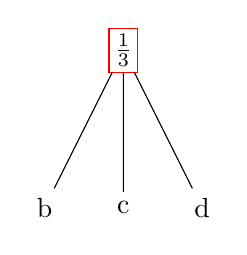
\begin{tikzpicture}%
  \tikzstyle{level 1}=[level distance=20mm,sibling distance=10mm]
  \tikzstyle{boxn}=[rectangle,draw=red,inner sep=2]
  \tikzstyle{cirn}=[circle,draw=blue,inner sep=1]
  \node(0)[boxn]{$\frac13$}
    child{node{b}}
    child{node{c}}
    child{node{d}}
    ;
\end{tikzpicture}
\quad
\begin{tikzpicture}%
  \tikzstyle{level 1}=[level distance=20mm,sibling distance=30mm]
  \tikzstyle{level 2}=[level distance=20mm,sibling distance=10mm]
  \tikzstyle{boxn}=[rectangle,draw=red,inner sep=2]
  \tikzstyle{cirn}=[circle,draw=blue,inner sep=1]
  \node(0)[boxn]{$\frac13$}
    child{node[cirn]{$\frac31$}
      child{node{e}} child{node{f}} child{node{g}}}
    child{node{c}}
    child{node{d}}
    ;
\end{tikzpicture}
\quad
\begin{tikzpicture}%
  \tikzstyle{level 1}=[level distance=20mm,sibling distance=30mm]
  \tikzstyle{level 2}=[level distance=20mm,sibling distance=10mm]
  \tikzstyle{boxn}=[rectangle,draw=red,inner sep=2]
  \tikzstyle{cirn}=[circle,draw=blue,inner sep=1]
  \node(0)[boxn]{$\frac13$}
    child{node[cirn]{$\frac31$}
      child{node{e}} child{node{f}} child{node{g}}}
    child{node[cirn]{$\frac21$}
      child{node{h}} child{node{i}}}
    child{node{d}}
    ;
\end{tikzpicture}
\quad
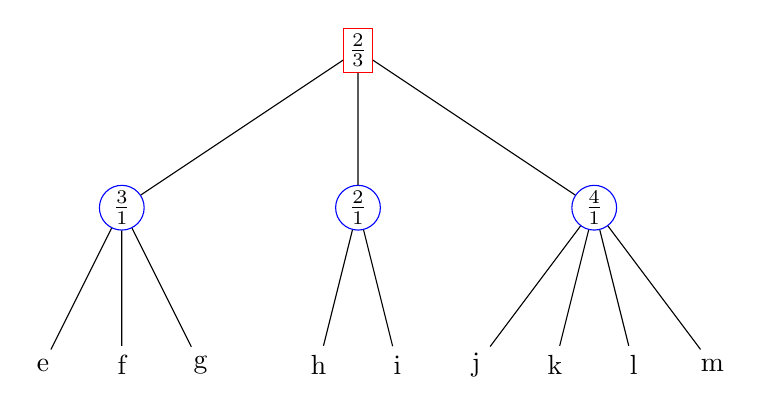
\begin{tikzpicture}%
  \tikzstyle{level 1}=[level distance=20mm,sibling distance=30mm]
  \tikzstyle{level 2}=[level distance=20mm,sibling distance=10mm]
  \tikzstyle{boxn}=[rectangle,draw=red,inner sep=2]
  \tikzstyle{cirn}=[circle,draw=blue,inner sep=1]
  \node(0)[boxn]{$\frac23$}
    child{node[cirn]{$\frac31$}
      child{node{e}} child{node{f}} child{node{g}}}
    child{node[cirn]{$\frac21$}
      child{node{h}} child{node{i}}}
    child{node[cirn]{$\frac41$}
      child{node{j}} child{node{k}} child{node{l}} child{node{m}}}
    ;
\end{tikzpicture}
\quad
\begin{tikzpicture}%
  \tikzstyle{level 1}=[level distance=20mm,sibling distance=40mm]
  \tikzstyle{level 2}=[level distance=20mm,sibling distance=15mm]
  \tikzstyle{level 3}=[level distance=20mm,sibling distance=5mm]
  \tikzstyle{boxn}=[rectangle,draw=red,inner sep=2]
  \tikzstyle{cirn}=[circle,draw=blue,inner sep=1]
  \node(0)[boxn]{$\frac23$}
    child{node[cirn]{$\frac31$}
      child{node{e}} child{node{f}} child{node{g}}}
    child{node[cirn]{$\frac21$}
      child{node[boxn]{$\frac12$} child{node{n}} child{node{o}}}
      child{node{i}}}
    child{node[cirn]{$\frac41$}
      child{node{j}} child{node{k}} child{node{l}} child{node{m}}}
    ;
\end{tikzpicture}
\quad
\begin{tikzpicture}%
  \tikzstyle{level 1}=[level distance=20mm,sibling distance=50mm]
  \tikzstyle{level 2}=[level distance=20mm,sibling distance=15mm]
  \tikzstyle{level 3}=[level distance=20mm,sibling distance=5mm]
  \tikzstyle{boxn}=[rectangle,draw=red,inner sep=2]
  \tikzstyle{cirn}=[circle,draw=blue,inner sep=1]
  \node(0)[boxn]{$\frac24$}
    child{node[cirn]{$\frac31$}
      child{node{e}} child{node{f}} child{node{g}}}
    child{node[cirn]{$\frac22$}
      child{node[boxn]{$\frac12$} child{node{n}} child{node{o}}}
      child{node[boxn]{$\frac13$} child{node{p}} child{node{q}} child{node{r}}}}
    child{node[cirn]{$\frac41$}
      child{node{j}} child{node{k}} child{node{l}} child{node{m}}}
    ;
\end{tikzpicture}
\quad
\begin{tikzpicture}%
  \tikzstyle{level 1}=[level distance=20mm,sibling distance=50mm]
  \tikzstyle{level 2}=[level distance=20mm,sibling distance=15mm]
  \tikzstyle{level 3}=[level distance=20mm,sibling distance=5mm]
  \tikzstyle{boxn}=[rectangle,draw=red,inner sep=2]
  \tikzstyle{cirn}=[circle,draw=blue,inner sep=1]
  \node(0)[boxn]{$\frac34$}
    child{node[cirn]{$\frac31$}
      child{node{e}} child{node{f}} child{node{g}}}
    child{node[cirn]{$\frac92$}
      child{node[boxn]{$\frac52$} child{node[cirn]{$\frac51$}} child{node[cirn]{$\frac71$}}}
      child{node[boxn]{$\frac43$} child{node[cirn]{$\frac41$}} child{node[cirn]{$\frac61$}} child{node[cirn]{$\frac81$}}}}
    child{node[cirn]{$\frac41$}
      child{node{j}} child{node{k}} child{node{l}} child{node{m}}}
    ;
\end{tikzpicture}
\quad
\begin{tikzpicture}%
  \tikzstyle{level 1}=[level distance=20mm,sibling distance=50mm]
  \tikzstyle{level 2}=[level distance=20mm,sibling distance=15mm]
  \tikzstyle{level 3}=[level distance=20mm,sibling distance=5mm]
  \tikzstyle{boxn}=[rectangle,draw=red,inner sep=2]
  \tikzstyle{cirn}=[circle,draw=blue,inner sep=1]
  \node(0)[boxn]{$\frac24$}
    child{node[cirn]{$\frac21$}
      child{node{$\frac0\infty$}} child{node{f}} child{node{g}}}
    child{node[cirn]{$\frac92$}
      child{node[boxn]{$\frac52$} child{node[cirn]{$\frac51$}} child{node[cirn]{$\frac71$}}}
      child{node[boxn]{$\frac43$} child{node[cirn]{$\frac41$}} child{node[cirn]{$\frac61$}} child{node[cirn]{$\frac81$}}}}
    child{node[cirn]{$\frac41$}
      child{node{j}} child{node{k}} child{node{l}} child{node{m}}}
    ;
\end{tikzpicture}
\quad
\begin{tikzpicture}%
  \tikzstyle{level 1}=[level distance=20mm,sibling distance=50mm]
  \tikzstyle{level 2}=[level distance=20mm,sibling distance=15mm]
  \tikzstyle{level 3}=[level distance=20mm,sibling distance=5mm]
  \tikzstyle{boxn}=[rectangle,draw=red,inner sep=2]
  \tikzstyle{cirn}=[circle,draw=blue,inner sep=1]
  \node(0)[boxn]{$\frac14$}
    child{node[cirn]{$\frac11$}
      child{node{$\frac0\infty$}} child{node{$\frac0\infty$}} child{node{g}}}
    child{node[cirn]{$\frac92$}
      child{node[boxn]{$\frac52$} child{node[cirn]{$\frac51$}} child{node[cirn]{$\frac71$}}}
      child{node[boxn]{$\frac43$} child{node[cirn]{$\frac41$}} child{node[cirn]{$\frac61$}} child{node[cirn]{$\frac81$}}}}
    child{node[cirn]{$\frac41$}
      child{node{j}} child{node{k}} child{node{l}} child{node{m}}}
    ;
\end{tikzpicture}
\quad
\begin{tikzpicture}%
  \tikzstyle{level 1}=[level distance=20mm,sibling distance=50mm]
  \tikzstyle{level 2}=[level distance=20mm,sibling distance=15mm]
  \tikzstyle{level 3}=[level distance=20mm,sibling distance=5mm]
  \tikzstyle{boxn}=[rectangle,draw=red,inner sep=2]
  \tikzstyle{cirn}=[circle,draw=blue,inner sep=1]
  \node(0)[boxn]{$\frac43$}
    child{node[cirn]{$\frac\infty0$}
      child{node{$\frac0\infty$}} child{node{$\frac0\infty$}} child{node{$\frac\infty0$}}}
    child{node[cirn]{$\frac92$}
      child{node[boxn]{$\frac52$} child{node[cirn]{$\frac51$}} child{node[cirn]{$\frac71$}}}
      child{node[boxn]{$\frac43$} child{node[cirn]{$\frac41$}} child{node[cirn]{$\frac61$}} child{node[cirn]{$\frac81$}}}}
    child{node[cirn]{$\frac41$}
      child{node{j}} child{node{k}} child{node{l}} child{node{m}}}
    ;
\end{tikzpicture}
\end{center}
\fi
...

\subsection{Modifications and enhancements}

Note that the proof-number algorithm (like the conspiracy numbers algorithm) works best on irregular
and non-uniformly branching trees --- if every node has exactly the same number of children and the
game-end nodes are all at the same distance from root, then the algorithm degenerates into a breadth-first
brute-force search.  

Transposition tables... GHI problem...


%%%%%%%%%%%%%%%%%%%%
\section{Other heuristics}

%%%%%%%%%%%%%%%%%%%%%%%%%%%%%%%%%%%%%%%%
%%%%%%%%%%%%%%%%%%%%%%%%%%%%%%%%%%%%%%%%
\chapter{Advanced Evaluation}
\label{chap-advanced-evaluation}

In this chapter we discuss the evaluation of

%%%%%%%%%%%%%%%%%%%%
\section{TDleaf($\lambda$)}
One of the most difficult aspects of constructing an evaluation function
can be ``tuning'' the weighting of different features.

Here we discuss a way for the computer to tune numeric parameters
(such as piece values) automatically.

\begin{enumerate}
\item Let $J(x,w)$ be a heuristic evaluation function parametrized by
  $w=(w_1,\dots,w_k)\in\mathbf{R}^k$.
\item Let $x_1,\dots,x_N$ be the positions that occurred in the game and let
  $x'_i$ be the leaf node of the principal variation of the search starting
  at $x_i$.
\item Let $r(x_N)\in\{\,-1,0,1\,\}$ be the outcome of the game.
\item Define $r(x_i',w)=\tanh(\beta\cdot J(x'_i,w))$, where $\beta=0.255$ for
  knightcap, (where $J$ is measured in units of 1 pawn).
\item For $i=1,\dots,N-1$ compute $d_i = r(x'_{i+1},w) - r(x'_i,w)$ and partial
  derivatives $\nabla r(x'_i,w) = (\dots \frac{\partial}{\partial w_j}r(x'_i,w) \dots)$.
\item If opponent rating is less than computer rating then set $d_i=0$ if the move
  leading to $x'_{i+1}$ was not predicted by the computer.
\item Update the parameters according to 
  \[ w'_j = w_j + \alpha \sum_{i=1}^{N-1} \frac{\partial}{\partial w_j} r(x'_i,w)
    \left( \sum_{m=i}^{N-1}\lambda^{m-i}d_m \right) \]
  where $\lambda$ is around 0.3--0.7 if the evaluation function is already reliable
  and $>0.95$ otherwise.  Choose $\alpha$ so that updates are about $1/100$ of a pawn.
\end{enumerate}

Remarks on evaluating the partial-derivative of the evaluation function: in some cases,
we may know the form of the evaluation and we can analytically derive the partial derivative.
But suppose we cannot do this easily (or we simply can't be bothered to do it).
A general approach to computing ...
\[ \frac{\partial}{\partial z}f(..., z, ...) \approx \frac{f(..., z+h, ...) - f(..., z-h, ...)}{2h} \]
for some small $h$ (but not too small).  This costs two computations of the evaluation function, but
works without special knowledge of the evaluation function ...

\subsection{TD($\mu$)}
The TD($\lambda$) algorithm suffers from the fact that it can learn to play
badly from bad examples.  The TD($\mu$) algorithm is a modification which is
designed to allow learning to happen even with bad examples.  This is especially
useful in the case of self-play; when there is no good opponent to practice and
learn from.

%%%%%%%%%%%%%%%%%%%%
\section{Neural networks}
Neural networks provide a way 

Neural networks have been used as components in various well-known and high-quality
game-engines, including NeuroGammon by ..., 

The down-side to neural networks is that executing them tends to be relatively slow, meaning that
they are not generally amenable to being used in a deep-searching approach which requires evaluating
millions of positions.

%%%%%%%%%%%%%%%%%%%%
\section{Genetic algorithms}
An interesting, but ...
Co-evolution ...
%%%%%%%%%%%%%%%%%%%%
\section{Pattern database / brains}

%%%%%%%%%%%%%%%%%%%%%%%%%%%%%%%%%%%%%%%%
%%%%%%%%%%%%%%%%%%%%%%%%%%%%%%%%%%%%%%%%
\chapter{GUI}
\label{chap-gui}

In this chapter we 

%%%%%%%%%%%%%%%%%%%%%%%%%%%%%%%%%%%%%%%%
%%%%%%%%%%%%%%%%%%%%%%%%%%%%%%%%%%%%%%%%
\chapter{Parallel Processing}
\label{chap-parallel}

Parallel processing is a technique that is important for taking advantage of the processing
power we have in current computers: from multi-core chips to massively-parallel GPUs to
networked workstations.  It is not straightforward to extend techniques such as \ab-search
to work efficiently in a parallel context.  There have been a number of

The biggest issue with parallel extensions of \ab-search is that the search is inherently
sequential: the results of search of one part of the tree is used when searching another, namely
the \ab-bounds.

%%%%%%%%%%%%%%%%%%%%
\section{Youngest Brothers Wait}

%%%%%%%%%%%%%%%%%%%%%%%%%%%%%%%%%%%%%%%%
%%%%%%%%%%%%%%%%%%%%%%%%%%%%%%%%%%%%%%%%
\chapter{Stuff}
\label{chap-stuff}

In this chapter we 

%%%%%%%%%%%%%%%%%%%%
\section{Notation}

\subsection{Forsythe-Edwards Notation (FEN)}
\subsection{GBR code}
\subsection{PGN}

%%%%%%%%%%%%%%%%%%%%
\section{Typesetting}

%%%%%%%%%%%%%%%%%%%%
\section{Ratings}
\subsection{Elo}
The Elo system (developed by Arpad Elo (?!)) is based on assigning numerical ratings to
players under the statistical assumption that the probability that a player with rating~$A$
will beat a player with rating~$B$ is given by
\[ \frac{10^{A/400}}{10^{A/400} + 10^{B/400}} = \frac{1}{1 + 10^{(B-A)/400}} \]
which means that a difference of 400 rating points corresponds to 10:1 odds in winning.

\subsection{Glicko}

%%%%%%%%%%%%%%%%%%%%
\section{Computer analysis}
\subsection{Blunder check}
\subsection{Auto-annotation}
\subsection{Combination finding}
\subsection{Automated problem construction}

%%%%%%%%%%%%%%%%%%%%%%%%%%%%%%%%%%%%%%%%
%%%%%%%%%%%%%%%%%%%%%%%%%%%%%%%%%%%%%%%%
\chapter{Opening Book}
\label{chap-opening}

In this chapter we discuss the usage and construction of an opening book.
\cite{buro}, \cite{donningerlorenz}

%%%%%%%%%%%%%%%%%%%%
\section{Basic format}

%%%%%%%%%%%%%%%%%%%%
\section{Basic usage}

\subsection{Hash approach}
One method (useful for small books with only positive entries)
is to simply store all positions
reachable from the book into the hash-table and when searching, if there
is a move which reaches a position in the table, to take one of such moves
(at random).  This approach will break down when you want to store moves
which should not be played, or if you want to associate probabilities or
other more sophisticated ...

%%%%%%%%%%%%%%%%%%%%
\section{Automatic construction}

%%%%%%%%%%%%%%%%%%%%
\section{Learning, updating}

%%%%%%%%%%%%%%%%%%%%%%%%%%%%%%%%%%%%%%%%
%%%%%%%%%%%%%%%%%%%%%%%%%%%%%%%%%%%%%%%%
\chapter{Endgame Tablebase}
\label{chap-endgame}

In this chapter we discuss the usage and construction of an endgame tablebase.

Note that the approach of endgame tablebases is not applicable to every game.  It works well
in the cases where the game ``simplifies'' towards the end of the game.  For example, if pieces
tend to get captured as the game goes on and there are fewer and fewer pieces on the board
(e.g. chess, checkers, mancala) then this approach works well.  If the position gets more complicated
as the game goes on (e.g. go, hex) or captured pieces are recycled (e.g. shogi)
then it may have limited utility.

%%%%%%%%%%%%%%%%%%%%
\section{Building}
The idea behind ...

The reason we use this backward approach of ``un-moving'' is to drastically reduce the amount
of computation we need to do.  Most positions in a given pass of the database will not be relevant,
so rather than evaluating all possible moves from all possible positions in a database to see
if they are a mate-in-$n$ position, we quickly scan through to find the (relatively) few
mate-in-$(n-1)$ positions and only for those positions we do a (un-)move generation step.
Though un-move-generation may be complex to code in a game, this can reduce computation time by
orders of magnitude (including reducing significantly the number of random-access hits to the
database being constructed --- this is important for cache behaviour in in-memory databases, as well
as disk-access speed in very large databases on disk.)

TODO:
simulate behaviour for naive ``forward-moving'' vs ``backward-moving'' for some simple game
(or congo for example? --- reusing existing code? --- can be for simple sub-game
LE+L, for example)
--- compute number of move-generations, random-accesses to database, overall clock-time.

\subsection{Thompson approach}

X. Thompson~\cite{thompson:endgame} gave an early algorithm for
``retrograde analysis of certain endgames''.  It uses 5 active bit-files (for small enough endgames,
they may fit entirely in memory and simply be bitmaps):
\begin{itemize}
  \item $W$: known white-to-move-and-win
  \item $B$: known black-to-move-and-lose
  \item $W_i$: latest white-to-move-and-win-in-$i$-moves
  \item $B_i$: latest black-to-move-and-lose-in-$i$-moves
  \item $J_i$: temporary work-file
\end{itemize}
Then the algorithm proceeds as follows:
\begin{itemize}
  \item[(Setup)]
    \begin{itemize}
      \item Set $B$ and $B_0$ to all positions with black to move but checkmated.
      \item Set $W=0$.
      \item Set $i=0$.
    \end{itemize}
  \item[(A)] For each $B_i$ position, generate predecessors --- add them to $W$
    and all positions not already in $W$ form the $W_{i+1}$ positions.
  \item[(B)] For each $W_{i+1}$ position, generate predecessors to $J_{i+1}$.
  \item[(C)] For each $J_{i+1}$ position, generate successors --- if all of them
    are in $W$ then the position is added to $B_{i+1}$.
    Finally, add $B_{i+1}$ to $B$.
  \item[(Loop)] Increment $i$ and iterate (A),(B),(C) until no changes to $B$ and $W$
\end{itemize}
\begin{verbatim}
  // Setup
  W = 0;
  B = B[0] = BlackCheckmated;
  ChangedB = ChangedW = true;
  for (i=0; ChangedB || ChangedW; ++i)
  {
    // (A)
    J = Predecessors(B[i]);
    W[i+1] = J & ~W;
    ChangedW = NonEmpty(W[i+1]);
    W = W | W[i+1];
    // (B)
    J = Predecessors(W[i+1]);
    // (C)
    B[i+1] = ProveSuccessors(J, W);
    ChangedB = !Subset(B[i+1], B);
    B = B | B[i+1];
  }
\end{verbatim}


\subsection{Wu-Beal approach}
Here we describe the algorithm given in \cite{wu-beal} for constructing endgame tablebases.
It is designed for handling large databases, minimizing what must be kept in main memory
(``random access'') ... fast sequential access disks ...
Thus we have the two full databases W/B accessed sequentially,
one working bitmap S accessed sequentially,
and only a single working bitmap R which must have random-access.
\begin{verbatim}
  // Set random-access bitmap R to predecessors of elements in sequential bitmap S
  R Predecessors(S);

  // load into S or R elements of W or B satisfying predicate P
  S/R Load(W/B, P);

  // Add elements of S to W or B with predicate P
  W/B Add(S, P);

  // Only keep elements of S with all successors in R
  S = ProveSuccessors(S,R)

  // W, B: full depth-to-win databases, accessed sequentially
  // S : sequential bitmap
  // R : random-access bitmap
  void toplevel()
  {
    do_initialize();
    N = 0;                            // depth to mate or conversion
    while (!done_white || !done_black)
    {
      if (!done_white)                // last pass added new positions
      {
        S = Load(W, WIN_IN(N));       // S = WTM win_in_n
        R = Predecessors(S);          // R = BTM predecessors of S
        S = Load(B, UNKNOWN);         // S = BTM unknown
        S = S & R;                    // S = BTM may lose_in_n
        R = Load(W, WIN_IN(<=N));     // R = WTM win_in_(n or less)
        S = ProveSuccessors(S,R);     // S = BTM lose_in_n
        B = Add(S, LOSE_IN(N));       // B += S
        if (distance_to_mate)         // distance_to_mate?
          S = LOAD(B, LOSE_IN(N));    // S = BTM lose_in_n
        R = Predecessors(S);          // R = WTM maybe win_in_(n+1)
        S = Load(W, UNKNOWN);         // S = WTM unknown
        S = S & R;                    // S = WTM win_in_(n+1)
        W = Add(S, WIN_IN_N(n+1));    // W += S
      }
      if (!done_black)                // done for BTM?
      {
        S = Load(B, WIN_IN(N));       // S = BTM win_in_n
        R = Predecessors(S);          // R = WTM predecessors of S
        S = Load(W, UNKNOWN);         // S = WTM unknown
        S = S & R;                    // S = WTM may lose_in_n
        R = Load(B, WIN_IN(<=N));     // R = BTM win_in_(n or less)
        S = ProveSuccessors(S,R);     // S = WTM lose_in_n
        W = Add(S, LOSE_IN(N));       // W += S
        if (distance_to_mate)         // distance_to_mate?
          S = LOAD(W, LOSE_IN(N));    // S = WTM lose_in_n
        R = Predecessors(S);          // R = BTM maybe win_in_(n+1)
        S = Load(B, UNKNOWN);         // S = BTM unknown
        S = S & R;                    // S = BTM win_in_(n+1)
        B = Add(S, WIN_IN_N(n+1));    // B += S
      }
    }
  }
\end{verbatim}

%%%%%%%%%%%%%%%%%%%%
\section{Encoding: symmetries and numbering}

An important technique for reducing the time and space complexity of the endgame tablebases
is the use of symmetries to collapse ``equivalent'' positions into a single entry.  A typical example
would be the \g{chess} endgame of King vs. King + Queen: one can rotate or reflect the board without
affecting the game-theoretic value of the positions, thus one could assum

Another technique to reduce the number of positions that needs to be considered is to take care to
eliminate impossible positions.  For example, in \g{chess}, 

%%%%%%%%%%%%%%%%%%%%
\section{Compressing}

Run-length encoding is a popular compression method that is well suited for sequential access to
a table.  It typically compresses significantly as many endgame tablebases consist of long runs
of draws.

Random-access into the table is much slower as one must scan through sequentially to find the appropriate
part of the table, though this can be sped up by the judicious use of indexes to point into the table.

%%%%%%%%%%%%%%%%%%%%
\section{Using}
(internal nodes, tradeoffs in search, etc.)

The API for accessing the database needs to be designed with these symmetries in mind.
And the search algorithm should be designed to interface with the endgame database in a transparent
manner that allows ...
Additionally, it is typically up to the ...
Allow fast first check if database exists...  then look up position


%%%%%%%%%%%%%%%%%%%%%%%%%%%%%%%%%%%%%%%%
%%%%%%%%%%%%%%%%%%%%%%%%%%%%%%%%%%%%%%%%
%%%%%%%%%%%%%%%%%%%%%%%%%%%%%%%%%%%%%%%%
%%%%%%%%%%%%%%%%%%%%%%%%%%%%%%%%%%%%%%%%
\part{Specific Games}

%%%%%%%%%%%%%%%%%%%%%%%%%%%%%%%%%%%%%%%%
%%%%%%%%%%%%%%%%%%%%%%%%%%%%%%%%%%%%%%%%
\chapter{Standard Models}
\label{chap-standard-models}

There are a couple classes of standard approaches (or ``models'') that
are applicable to 


%%%%%%%%%%%%%%%%%%%%
\section{\ab-search}

Our standard approach, which we will call the {\em \ab-search model},
(applicable to most chess-like games) is as follows: negamax search with \ab-pruning, iterative-deepening,
transposition tables, quiescence search (where applicable), null-move pruning. [PVS search?]
The static evaluation functions will depend heavily on the game in question but will be
tuned using the TDLeaf($\lambda$) algorithm.

Endgame tablebases will be built where applicable using retrograde analysis.

Opening books constructed using ...

The standard time-management approach will be used.


%%%%%%%%%%%%%%%%%%%%
\section{MCTS}

Another standard approach, which has proven effective for some games, such as \g{go} and \g{hex},
is the {\em MCTS model}: a Monte-Carlo tree search based on UCT with modifications to incorporate
domain-specific knowledge and with progressive widening.

%%%%%%%%%%%%%%%%%%%%
\section{Etc.}

non-deterministic games

incomplete information

multi-player games

Arimaa...


%%%%%%%%%%%%%%%%%%%%%%%%%%%%%%%%%%%%%%%%
%%%%%%%%%%%%%%%%%%%%%%%%%%%%%%%%%%%%%%%%
\chapter{Congo}
\label{chap-congo}

In this chapter we delve more deeply into the game of \g{congo}.

We will apply our standard approach of \ab-search with
iterative deepening, transposition table and quiescence extensions (based on captures,
checks, and drowning.)
For static evaluation we'll use material values with a piece-square bonus as well
as some \g{congo}-specific features such as TODO

We'll use the TDLeaf($\lambda$) self-learning approach to arrive at the appropriate
weightings.

For end-games, we'll go ahead and build 3, 4, and 5-piece table-bases.

Opening books will be built by the self-play and deep-search approach.

--- lion, pawn, super-pawn, elephant, monkey, alligator, giraffe

\section{Endgame Tablebase}

We will build end-game tablebases for all endings with up to 4 pieces (plus lions).
First, let's estimate the number of positions in endgames of the different types.
A few remarks are in order here: first, since the lions are restricted to their $3\x3$ dens, there are
at most 81 positions for the pairs of lions to be in, and we will assume that the white lion
is in the left-most 6 squares in his den, giving us only $6\x9=54$ different lion dispositions.
The pawn cannot occur in the last row (since it will promote when it reaches the last line), giving
only $7\x6-2=40$ possible positions (2 of the squares are occupied by lions).  For other piece types, there
are no restrictions except for the general restrictions of only one piece per square, giving $49-n$ possible
squares, where $n$ is the number of occupied.
\[\begin{array}{lccc}
\text{L+L} & & 54 & 54 \\
\text{LP+L} & 54\x40 & 2160 & 2214 \\
\text{LX+L (x=S/E/M/A/G)} & 54\x(49-2)& 12\,690 \text{(2538 each)} & 14\,904 \\
\text{LP+LP} & 54\x40\x(40-1) & 84240 & 99\,144 \\
\text{LX+LP (x=S/E/M/A/G)} & 54\x(49-2)\x(40-1)\x5& 494\,910 \text{(98\,982 each)} & 594\,054 \\
\text{LX+LX (x=S/E/M/A/G)} & 54\x(49-2)\x(49-3)\x5& \\
\text{LX+LY (x,y=S/E/M/A/G;x$\neq y$)} & 54\x(49-2)\x(49-3)\x5\x4& \\
\text{LXP+L (x=S/E/M/A/G)} & 54\x(49-2)\x(40-1)\x5& 494\,910 \text{(98\,982 each)} & \\
\text{LXY+L (x,y=S/E/M/A/G)} & 54\x(49-2)\x(49-3)\x5\x5& 2\,918\,700 \text{(116\,748 each)} & \\
\end{array}\]

The simplest encoding gives for each particular man-combination:
\[\begin{array}{lccc}
\text{L+L} & 9\x9 & 81 & 81 \\
\text{LX+L (x=P/S/E/M/A/G)} & 9\x9\x49\x6 & 23\,814 \text{(3969 each)} & 23\,895 \\
\text{LXY+L (x,y=P/S/E/M/A/G)} & 9\x9\x49^2\x6^2 & 7\,001\,316 \text{(194\,481 each)} & 7\,025\,211 \\
\text{LX+LY (x,y=P/S/E/M/A/G)} & 9\x9\x49^2\x6^2 & 7\,001\,316 \text{(194\,481 each)} & 14\,026\,527 \\
\text{LXY+LZ (x,y,z=P/S/E/M/A/G)} & 9\x9\x49^3\x6^3 & 2\,058\,386\,904 \text{(9\,529\,569 each)} \\
\text{LXYZ+L (x,y,z=P/S/E/M/A/G)} & 9\x9\x49^3\x6^3 & 2\,058\,386\,904 \text{(9\,529\,569 each)} \\
\end{array}\]

\subsection{Another attempt at counting endgame positions (10-20-2011)}

Note that we can choose either a lion {\em or} a piece to be restricted to, say, the left side
of the board.  To indicate which piece is restricted, we use underlining below.  Note also that pawns
cannot be in the first or last rows.
\[\begin{array}{lccc}
\text{\underline{L}L} & 6\x9 & 54 & 54 \\
\text{L\underline{X}L (x=ACEGSZ)} & 81\x28 & 13,608 \text{(2,268 each)} &  \\
\text{L\underline{P}L} & 81\x20 & 1,620 &  \\
\text{L\underline{X}LY (x,y=ACEGSZ)} & 81\x28\x46 & 2,190,888 \text{(104,328 each)} & \\
\text{L\underline{X}YL (x,y=ACEGSZ; x<y)} & 81\x28\x46 & 1,564,920 \text{(104,328 each)} & \\
\text{L\underline{X}XL (x=ACEGSZ)} & 54\x\frac{47\x46}{2} & 350,244 \text{(58,374 each)} & \\
\text{L\underline{X}LP (x=ACEGSZ)} & 81\x28\x35 & 476,280 \text{(79,380)} & \\
\text{L\underline{X}PL (x=ACEGSZ)} & 81\x28\x35 & 476,280 \text{(79,380)} & \\
\text{L\underline{P}LP} & 81\x20\x34 & 55,080 & \\
\text{L\underline{P}PL} & 81\x20\x34 & 55,080 & \\
\text{\underline{L}XXLY (x,y=ACEGSZ)} & 54\x\frac{47\x46}{2}\x45 & 94,565,880 \text{(2,626,830 each)} & \\
\text{L\underline{X}YLZ (x,y,z=ACEGSZ; x<y)} & 81\x28\x46\x45 & 422,528,400 \text{(4,694,760 each)} & \\
\end{array}\]


%%%%%%%%%%%%%%%%%%%%%%%%%%%%%%%%%%%%%%%%
%%%%%%%%%%%%%%%%%%%%%%%%%%%%%%%%%%%%%%%%
\chapter{Mancala}
\label{chap-mancala}

In this chapter we delve more deeply into the sowing game of \g{mancala}.  Now, there
are many different variants of this game; indeed, one might rather call this a
{\em family} of games, rather than a game.  Examples include
\g{owari}, \g{mancala}, \g{kalah}, \g{bao}, ...

\section{Kalah}
Kalah 
\section{Awari}
\section{Mancala}
\section{Dakon}
\section{Bao}

%%%%%%%%%%%%%%%%%%%%%%%%%%%%%%%%%%%%%%%%
%%%%%%%%%%%%%%%%%%%%%%%%%%%%%%%%%%%%%%%%
\chapter{Chess}
\label{chap-chess}

In this chapter we delve more deeply into the game of \g{chess}.

%%%%%%%%%%%%%%%%%%%%%%%%%%%%%%%%%%%%%%%%
%%%%%%%%%%%%%%%%%%%%%%%%%%%%%%%%%%%%%%%%
\chapter{Checkers}
\label{chap-checkers}

In this chapter we delve more deeply into the game of \g{checkers}.

\g{checkers} is an old game

\g{checkers} is solved --- that it is known to be a theoretical draw.

\g{checkers} is 

%%%%%%%%%%%%%%%%%%%%%%%%%%%%%%%%%%%%%%%%
%%%%%%%%%%%%%%%%%%%%%%%%%%%%%%%%%%%%%%%%
\chapter{Xiangqi}
\label{chap-xiangqi}

In this chapter we delve more deeply into the game of \g{xiangqi} (or \g{chinese chess}).

%%%%%%%%%%%%%%%%%%%%%%%%%%%%%%%%%%%%%%%%
%%%%%%%%%%%%%%%%%%%%%%%%%%%%%%%%%%%%%%%%
\chapter{Sh\=ogi}
\label{chap-shogi}

In this chapter we delve more deeply into the game of \g{sh\=ogi} and some of its
many variations.

%%%%%%%%%%%%%%%%%%%%%%%%%%%%%%
\section{Sh\=ogi}
\label{sec-shogi}

the game of \g{sh\=ogi}.

%%%%%%%%%%%%%%%%%%%%%%%%%%%%%%
\section{D\=obutsu sh\=ogi}
\label{sec-dobutsu-shogi}

the game of \g{d\=obutsu sh\=ogi}.

%%%%%%%%%%%%%%%%%%%%%%%%%%%%%%
\section{Tori sh\=ogi}
\label{sec-tori-shogi}

the game of \g{tori sh\=ogi}.

%%%%%%%%%%%%%%%%%%%%%%%%%%%%%%
\section{Poppy sh\=ogi}
\label{sec-poppy-shogi}

the game of \g{poppy sh\=ogi}.

%%%%%%%%%%%%%%%%%%%%%%%%%%%%%%
\section{Whale sh\=ogi}
\label{sec-whale-shogi}

the game of \g{whale sh\=ogi}.

%%%%%%%%%%%%%%%%%%%%%%%%%%%%%%
\section{Chu sh\=ogi}
\label{sec-chu-shogi}

The game of \g{chu sh\=ogi} is a fascinating
game that was ... china... 15th century... with ...

The biggest problem it will present is simply one of scale ---
the game is played on a $12\x12$ board and there are ... pieces
on the board at the start of the game.  This gives a large branching
factor, implying that it will be difficult to search very deeply;
but ...

%%%%%%%%%%%%%%%%%%%%%%%%%%%%%%
\section{Tenjiku sh\=ogi}
\label{sec-tenjiku-shogi}

The game of \g{tenjiku sh\=ogi} is similar to \g{chu sho\=ogi} but is
even larger: it is played on 

Despite its large size, it has a highly tactical flavor 

%%%%%%%%%%%%%%%%%%%%%%%%%%%%%%%%%%%%%%%%
%%%%%%%%%%%%%%%%%%%%%%%%%%%%%%%%%%%%%%%%
\chapter{Tafl}
\label{chap-tafl}

In this chapter we delve more deeply into the game of \g{hnefatafl}.  This is
an ancient game and not without interest.  Due to its venerability there is a
high degree of variability in rules and many variations and variants.

The specific variation we will cover here is ... 

%%%%%%%%%%%%%%%%%%%%%%%%%%%%%%
\section{Evaluation}

One component of an evaluation function we will use for this game is the number
of consecutive moves it would take the king to win.  

%%%%%%%%%%%%%%%%%%%%%%%%%%%%%%
\section{Mate search}

This game seems ideal for approaches such as proof-number search or $\lambda$-search.

%%%%%%%%%%%%%%%%%%%%%%%%%%%%%%%%%%%%%%%%
%%%%%%%%%%%%%%%%%%%%%%%%%%%%%%%%%%%%%%%%
\chapter{Go}
\label{chap-go}

In this chapter we delve more deeply into the game of \g{go} (or \g{weiqi}).

%%%%%%%%%%%%%%%%%%%%%%%%%%%%%%%%%%%%%%%%
%%%%%%%%%%%%%%%%%%%%%%%%%%%%%%%%%%%%%%%%
\chapter{Havannah}
\label{chap-havannah}

In this chapter we delve more deeply into the game of \g{havannah}.

For this game, MCTS (with various modifications) has proven to be highly effective.

%%%%%%%%%%%%%%%%%%%%%%%%%%%%%%%%%%%%%%%%
%%%%%%%%%%%%%%%%%%%%%%%%%%%%%%%%%%%%%%%%
\chapter{Hex}
\label{chap-hex}

In this chapter we delve more deeply into connection games, in particular
the game of \g{hex}.

%%%%%%%%%%%%%%%%%%%%%%%%%%%%%%%%%%%%%%%%
%%%%%%%%%%%%%%%%%%%%%%%%%%%%%%%%%%%%%%%%
\chapter{Hive}
\label{chap-hive}

In this chapter we delve more deeply into the game of \g{hive}.

\g{hive} presents some new complications for programming.  It has
no set board --- in principle it is played on an infinite board.
That is, since the pieces are placed ...



%%%%%%%%%%%%%%%%%%%%%%%%%%%%%%%%%%%%%%%%
%%%%%%%%%%%%%%%%%%%%%%%%%%%%%%%%%%%%%%%%
\chapter{Amazons}
\label{chap-amazons}

In this chapter we delve more deeply into the game of \g{amazons}.

%%%%%%%%%%%%%%%%%%%%%%%%%%%%%%%%%%%%%%%%
%%%%%%%%%%%%%%%%%%%%%%%%%%%%%%%%%%%%%%%%
\chapter{Dots-and-boxes}
\label{chap-dots-and-boxes}

In this chapter we delve more deeply into the game of \g{dots-and-boxes}.

%%%%%%%%%%%%%%%%%%%%%%%%%%%%%%%%%%%%%%%%
%%%%%%%%%%%%%%%%%%%%%%%%%%%%%%%%%%%%%%%%
\chapter{Exotica}
\label{chap-exotica}

%%%%%%%%%%%%%%%%%%%%
\section{Backgammon}
The game of \g{backgammon} represents new challenges, the biggest being that of
randomness --- usage of dice complicates matters.

%%%%%%%%%%%%%%%%%%%%
\section{Poker}
The game of \g{poker} represents many new challenges.  In addition to the randomness
of the shuffled deck, we also have imperfect information: we don't know
what cards the other players are holding.

%%%%%%%%%%%%%%%%%%%%
\section{Kriegspiel, Stratego}
The games \g{kriegspiel} and \g{stratego} represents the challenges of

%%%%%%%%%%%%%%%%%%%%
\section{Wargames, Advanced Squad Leader}
The game \g{advanced squad leader} (ASL) 

%%%%%%%%%%%%%%%%%%%%%%%%%%%%%%%%%%%%%%%%
%%%%%%%%%%%%%%%%%%%%%%%%%%%%%%%%%%%%%%%%
\chapter{Combinatorial game theory}
\label{chap-cgt}

In this chapter we discuss 

%%%%%%%%%%%%%%%%%%%%%%%%%%%%%%%%%%%%%%%%
%%%%%%%%%%%%%%%%%%%%%%%%%%%%%%%%%%%%%%%%
\chapter{Zillions of Games}
\label{chap-zog}

Zillions of Games is a game package for Windows that uses a ``universal gaming engine''
technology that allows you to play nearly any abstract board game or puzzle in the world.

%%%%%%%%%%%%%%%%%%%%%%%%%%%%%%%%%%%%%%%%
%%%%%%%%%%%%%%%%%%%%%%%%%%%%%%%%%%%%%%%%
\chapter{International Computer Olympiada (ICGA)}

\begin{tabular}{lcc}
\bf Game  &\bf Tournaments  &\bf Programs \\\hline
\g{abalone}  &1  &2 \\
\g{amazons}  &9  &12 \\
\g{awari}  &5  &9 \\
\g{backgammon}  &7  &12 \\
\g{bridge}  &5  &9 \\
\g{checkers}  &2  &8 \\
\g{chess}  &60  &245 \\
\g{chinese Chess}  &13  &36 \\
\g{clobber}  &2  &3 \\
\g{connect6}  &4  &17 \\
\g{connect-four}  &1  &4 \\
\g{dominoes}  &1  &3 \\
\g{dots and boxes}  &4  &8 \\
\g{draughts}  &9  &21 \\
\g{ginrummy}  &1  &2 \\
\g{gipf}  &1  &2 \\
\g{go}  &25  &59 \\
\g{go-moku}  &4  &16 \\
\g{havannah}  &1  &2 \\
\g{hex}  &6  &9 \\
\g{kriegspiel}  &2  &4 \\
\g{lines of action}  &7  &9 \\
\g{nine men's morris}  &1  &2 \\
\g{octi}  &1  &2 \\
\g{othello}  &4  &31 \\
\g{phantom Go}  &3  &4 \\
\g{poker}  &1  &2 \\
\g{pool}  &3  &6 \\
\g{qubic}  &2  &4 \\
\g{renju}  &4  &9 \\
\g{scrabble}  &4  &8 \\
\g{shogi}  &9  &10 \\
\g{surakarta}   &2  &3
\end{tabular}

\section{2008 Computer Olympiad (call for participation)}
Official games:

\g{abalone}, \g{amazons}, \g{arimaa}, \g{backgammon}, \g{bao}, \g{bridge},
\g{chinese chess}, \g{clobber}, \g{computational pool}, \g{connect-6},
\g{diplomacy}, \g{dominoes}, \g{dots-and-boxes}, \g{10x10 draughts},
\g{gipf}, \g{go}, \g{9x9 go}, \g{hex}, \g{kriegspiel}, \g{lines of action},
\g{octi}, \g{othello}, \g{phantom go}, \g{poker}, \g{scrabble}, \g{stratego},
\g{shogi}, \g{surakarta}

Willing to host more if there were strong engines, such as:

\g{ataxx}, \g{dvonn}, \g{mediocrity}, \g{onyx}, \g{tamsk}, \g{twixt}, \g{z\`ertz}

\section{2009 Computer Olympiad (competed)}
\g{amazons}, \g{chess}, \g{chinese chess}, \g{connect6}, \g{draughts},
\g{go}, \g{go (9x9)}, \g{hex}, \g{lines of action}, \g{shogi},
\g{havannah}, \g{kriegspiel}, \g{phantom go}

\section{2010 Computer Olympiad}

\subsection{call for participation}
\g{amazons}, \g{backgammon}, \g{bridge}, \g{chess}, \g{computational pool}, \g{connect6},
\g{chinese chess}, \g{dots and boxes}, \g{international draughts}, \g{19x19 go},
\g{9x9 go}, \g{hex}, \g{havannah}, \g{lines of action}, \g{sh\=ogi}, and, \g{surakarta}

\subsection{participated}

%%%%%%%%%%%%%%%%%%%%%%%%%%%%%%%%%%%%%%%%
%%%%%%%%%%%%%%%%%%%%%%%%%%%%%%%%%%%%%%%%
\chapter{Game rules, sample games, comparisons}

\begin{tabular}{lrrrr}
Game & Average game length & Average number of moves & Estimated State Space
& Classifications \\\hline
Checkers & & & \\
Chess & & & \\
Awari & & & \\
Shogi & & & \\
Go & & & \\
Amazons & & & \\
Shogi & & & \\
\end{tabular}
Classification codes: 
Endgame: convergent/divergent/stationary
Information: perfect/imperfect(common)/imperfect(private)
Determinism: deterministic/stochastic


\g{chess}, \g{checkers}, \g{chinese chess}, \g{shogi},
\g{congo}, \g{go}, \g{hex}, \g{dots-and-boxes}, \g{amazons},
\g{mancala}/\g{awari}, \g{backgammon}, \g{connect-4}, \g{phutball},
\g{tafl}/\g{tablut}, \g{othello}, \g{konane}, \g{fox-and-geese},
\g{nine-man-morris},

\g{khet}, \g{abalone}, 

\g{yavalath}, \g{pentalath}, \g{patagonia},  (Browne's games)

\g{gipf}, \g{yinsh}, \g{tzaar}, \g{z\'ertz}, \g{dvonn}, \g{p\"unct},

\g{bridge}, \g{poker}, \g{scrabble}, \g{monopoly}, \g{kriegspiel},
\g{yahtzee}, \g{stratego},

settlers of cataan, carcasonne, puerto rico,
yahtzee, parchisi, clue(do), 

{\it  Encyclopedia of Chess Variants}:
progressive chess, alapo, alice chess, atomic chess, avalanche chess,
barrier chess I, beirut chess, berolina chess, betza's chess, bird chess I, bomb chess,
caissa, carnivore chess, chad,
checkless chess, chess football, chezz, chu shogi,
columbia common chess, congo, diana, dragon chess, dragonfly,
eternity's children, extinction chess,
grand chess, hexagonal chess (glinski's), jetan,
kamikaze chess I, koopa chess, loonybird, losing chess, makruk,
microchess I/II/III/IV, mimic chess I/II, minishogi,
missile chess, rifle chess, null chess, one-dimensional chess,
parallel time-stream chess (?), parallel world chess, the pawn's game I,
petty chess, ploy, rotary, plague chess, push chess, quest-chess,
quickchess, refusal chess, compromise chess, sjakti, smess, spite chess,
star-trek chess, three kings chess, tori shogi, tenjiku shogi,
ultima, wa shogi, whale shogi, yari shogi

\cite{heinz00}

\section{Congo}
\g{congo} is a chess-like game played on an $7\x7$ board with 

\section{Chess}
\g{chess} is played on an $8\x8$ board with 

%\setchessboard{smallboard,showmover=false}
%\newchessgame
%\chessboard

\newcommand{\boardthreebythree}[9]{
\setlength{\unitlength}{1mm}
\begin{picture}(15,15)(0,0)
\put(0,5){\line(1,0){15}}
\put(0,10){\line(1,0){15}}
\put(5,0){\line(0,1){15}}
\put(10,0){\line(0,1){15}}
\thicklines
\put(0,0){\line(1,0){15}}
\put(0,0){\line(0,1){15}}
\put(15,0){\line(0,1){15}}
\put(0,15){\line(1,0){15}}
\put(0,10){\makebox(5,5){#1}}
\put(5,10){\makebox(5,5){#2}}
\put(10,10){\makebox(5,5){#3}}
\put(0,5){\makebox(5,5){#4}}
\put(5,5){\makebox(5,5){#5}}
\put(10,5){\makebox(5,5){#6}}
\put(0,0){\makebox(5,5){#7}}
\put(5,0){\makebox(5,5){#8}}
\put(10,0){\makebox(5,5){#9}}
\end{picture}
}
    \boardthreebythree{1}{2}{3}{4}{5}{6}{7}{8}{9}
The pieces' basic movement is given as follows
\begin{itemize}
\item King - moves one step in any direction \\
    \boardthreebythree{$\x$}{$\x$}{$\x$}{$\x$}{K}{$\x$}{$\x$}{$\x$}{$\x$}
\item Queen - slides any number of steps in any direction \\ 
    \boardthreebythree{$\nwarrow$}{$\uparrow$}{$\nearrow$}{$\leftarrow$}{Q}{$\rightarrow$}{$\swarrow$}{$\downarrow$}{$\searrow$}
\item Rook - slides any number of steps in an orthogonal direction \\ 
    \boardthreebythree{}{$\uparrow$}{}{$\leftarrow$}{R}{$\rightarrow$}{}{$\downarrow$}{}
\item Bishop - slides any number of steps in a diagonal direction \\ 
    \boardthreebythree{$\nwarrow$}{}{$\nearrow$}{}{B}{}{$\swarrow$}{}{$\searrow$}
\item Knight - jumps one orthogonal and one diagonal step \\ 
    $\begin{array}{||c|c|c|c|c||}\hline\hline
   & \x &          & \x &    \\\hline
\x &    &          &    & \x \\\hline
   &    & \text{N} &    &    \\\hline
\x &    &          &    & \x \\\hline
   & \x &          & \x &    \\\hline\hline
\end{array}$
\item Pawn - moves one step forward (without the right of capturing) or captures diagonally forward \\
    \boardthreebythree{$c$}{$m$}{$c$}{}{P}{}{}{}{}
\end{itemize}

\section{Shogi}

%%%%%%%%%%%%%%%%%%%%%%%%%%%%%%%%%%%%%%%%
%%%%%%%%%%%%%%%%%%%%%%%%%%%%%%%%%%%%%%%%
\chapter*{Glossary}
\addcontentsline{toc}{chapter}{Glossary}

\newcommand{\gloss}[2]{\par{\bf{#1}} --- {#2}}

\gloss{PNS}{see proof-number search}
\gloss{proof-number search}{A method of searching}

%%%%%%%%%%%%%%%%%%%%%%%%%%%%%%%%%%%%%%%%
%%%%%%%%%%%%%%%%%%%%%%%%%%%%%%%%%%%%%%%%
%\chapter{Index}
\newpage
\addcontentsline{toc}{chapter}{Index}
\printindex

%%%%%%%%%%%%%%%%%%%%%%%%%%%%%%%%%%%%%%%%
%%%%%%%%%%%%%%%%%%%%%%%%%%%%%%%%%%%%%%%%
%\chapter{Bibliography}
\bibliographystyle{amsalpha}
\cleardoublepage
\addcontentsline{toc}{chapter}{Bibliography}
\bibliography{book-bib}

%%%%%%%%%%%%%%%%%%%%%%%%%%%%%%%%%%%%%%%%%%%%%%%%%%%%%%%%%%%%
%%%%%%%%%%%%%%%%%%%%%%%%%%%%%%%%%%%%%%%%%%%%%%%%%%%%%%%%%%%%
\end{document}
%%%%%%%%%%%%%%%%%%%%%%%%%%%%%%%%%%%%%%%%%%%%%%%%%%%%%%%%%%%%
%%%%%%%%%%%%%%%%%%%%%%%%%%%%%%%%%%%%%%%%%%%%%%%%%%%%%%%%%%%%
